\documentclass[acmsmall]{acmart}
\usepackage{multicol,lipsum}
\usepackage{tikz}
\usepackage{graphicx}
\usetikzlibrary{arrows, positioning, automata, shapes}
\usepackage{amsfonts}
\usepackage{mathrsfs}
\usepackage{booktabs}
\usepackage{amsmath, colortbl}
\usepackage{listings} % Code listings, with syntax highlighting
\usepackage{hyperref}
\setcopyright{none}
\settopmatter{printacmref=false}
\renewcommand\footnotetextcopyrightpermission[1]{}
\pagestyle{plain}

\begin{document}
\title{MSDS 6372 Project 1}
\author{Samuel Arellano}
\email{sarellano@mail.smu.edu}
\author{Travis Daun}
\email{trdaun@mail.smu.edu}
\affiliation{
	\institution{Applied Statistics:Inference and Modeling, MSDS6372, Southern Methodist University}
}


\begin{abstract}

\end{abstract}

\maketitle


\thispagestyle{plain}
\section{Introduction}
Since Toyota’s introduction of the Prius in 1997, there has been great interest in hybrid electric vehicles (HEVs) and a growing adoption of these vehicles by consumers. This has spurred other auto manufacturers to release their own versions of alternative fuel vehicles and led to a wide variety of HEVs for consumers to choose from. While the feature that consumers typically look for, and the one most marketed by manufacturers, is that of fuel efficiency measured in mile per gallon (MPG), one feature often overlooked is acceleration. Acceleration is not only an important performance metric, but like MPG, increases in acceleration rates of a vehicle class can be an indicator of technological advancement. In this study will review HEV data to determine what vehicle characteristics most influence a vehicle’s acceleration rates, attempt to create a model based on the data that accurately predicts acceleration, and determine if acceleration rates across various classes of automobiles have improved over time.
\section{Data Description}
The dataset is composed of 153 observations.  Each observation is distinct model year HEV consisting of 9 variables (carid, vehicle, year, msrp, accelrate, mpg, mpgmpge, carclass, carclass\_id). Each observation is identified by a unique carid. The HEV model is defined by the variable vehicle. Model year is defined by year. MSRP refers to the manufacturer's suggested retail price normalized to 2013 dollars. The acceleration rate is recorded as accelrate and represents the time in seconds required for the vehicle to reach a speed of 60 mph from a complete stop. Fuel economy is measured by the variable MPG. The variable MPGMPGe records the higher of the vehicles MPG or MPG equivalent estimated as $MPG_e = \frac{33.7 \times \text{driving range}}{\text{battery capacity}}$. The vehicles are categorized into 7 classes (C = Compact, M = Midsize, TS = 2 Seater, L = Large, PT = Pickup Truck, MV = Minivan, SUV = Sport Utility Vehicle) denoted under the variable carclass and each class is assigned a number denoted under the variable carclass\_id. \\

\noindent Dataset: hybrid\_reg.csv\\
Source: D-J. Lim, S.R. Jahromi, T.R. Anderson, A-A. Tudorie (2014). “Comparing Technological Advancement of Hybrid Electric Vehicles (HEV) in Different Market Segments,” Technological Forecasting \& Social Change, http://dx.doi.org/10.1016/j.techfore.2014.05.008

\section{Exploratory Analysis}
After an initial review of the data it was determined that the variable carid would not be used in linear modeling as its sole purpose was the identification of observations and because the vehicles were ordered by year and carid was assigned incrementally, using carid would invariably lead to collinearity problems with year without adding any information of value. \\

The categorical variables, \texttt{vehicles} and \texttt{carclass\_id} were tested against \texttt{accelrate} to determine if the differences in mean acceleration rates were significantly different when grouped by model or car class. We found that using an analysis of variance, the effect of vehicle was significant with a p-value of <.0001 and its R-Square value of .953 suggested that it might be a good explanatory variable, this can be seen in Figure~\ref{fig:ABV} . Similarly, as seen in Figure~\ref{fig:ABCC} we found the effect of \texttt{carclass\_id} was statistically significant with a p-value of <.0001, though at .337 it had a lower R-Squared value. \\

To test the fit of the continuous variables, we ran a scatterplot matrix and color coded the plots by car class. As can be seen in Figure~\ref{fig:SCAT}, visual analysis of the scatterplot matrix indicated a normal distribution of the response variable \texttt{accelrate} and the presence of a good linear correlation between \texttt{accelrate} and \texttt{msrp}. It also indicated that there might be a linear correlation between \texttt{accelrate} and \texttt{year} if controlled for \texttt{carclass}. In Figure~\ref{fig:HCDPC}, we suspected that there might be a curvilinear relationship between \texttt{accelrate} and the variables \texttt{mpg} and \texttt{mpgmpge}, however after transforming the variables we decided that what we were seeing was the presence of outliers and not an indication of a nonlinear relationship. We performed a logarithmic transformation of \texttt{mpg} and \texttt{mpgmpge} to see if it would help improve linearity. We found that while the transformation made a marginal improvement on linear correlation and the logged values were more normally distributed, the improvement was not enough to warrant altering the data and since normal distribution of the predictor variables is not necessary for conducting a multiple regression, we opted to move forward with non-transformed data. This can be seen in Figure~\ref{fig:TFPC} and Figure~\ref{fig:TFLAPC}. Analysis of the scatter plots also revealed the presence of collinearity between \texttt{year} and \texttt{carid} and between \texttt{mpg} and \texttt{mpgmpge}. The strong relation between \texttt{carid} and \texttt{year} was expected due to the data being sorted by year prior to the sequential assignment of car identification numbers. Due to the small quantity of all-electric HEV’s, nearly all observations of \texttt{mpg} and \texttt{mpgmpge} were the same, resulting in strong collinearity between the two variables. \\

It was also important to understand the interactions between the various predictors. Figure~\ref{fig:INTMPG} shows how the interaction between \texttt{mpg} and \texttt{carclass} impacts \texttt{accelrate}. We asked ourselves two main questions when exploring interactions; 1) Does the interaction make sense, and 2) Is the interaction statistically significant? For the interaction between \texttt{carclass} and \texttt{mpg} we determined that yes, some interaction would make sense, but as can be seen in Figure~\ref{fig:INTMPG} the interaction is not statistically significant.  We also explored the interaction between \texttt{carclass} and \texttt{msrp} which can be seen in Figure~\ref{fig:INTMSRP}. Again intuition told us that this interaction makes conceptual sense since car prices are greatly impacted by the type of car you are buying. Again when the statistical significance of this interaction is explored, Figure~\ref{fig:INTMSRP} shows that the interaction between \texttt{carclass} and \texttt{msrp} are not statistically significant.\\

Because the value of \texttt{carid} has no real effect on the question of interest we decided to go ahead and remove it from further analysis. We then had to decide if we wanted to proceed with either \texttt{mpg} or \texttt{mpgmpge} in linear modeling. From the correlation matrix we found that the Pearson Correlation Coefficients of \texttt{mpg} and \texttt{mpgmpge} were -.506 and -.399 respectively, so we decided to explore mpg further as we moved into linear modeling. Before moving on we decided to run more correlation tests and explored various transformations of mpg against accelrate to ensure that our previous conclusion that the apparent curve in the line was nothing more than the presence of outliers. With the exploratory data analysis complete we moved on to linear modeling. 

\section{Objective 1}
\subsection{Restatement of Problem and the overall approach to solve it}
We wanted to determine if the acceleration rate of a HEV could be predicted by the price paid for the car, the miles per gallon that the car achieved, and the year that the car was manufactured. We chose to apply a multiple linear regression models using various sub set selection techniques. Specifically we employed stepwise, least angle regression (LAR), and least absolute shrikage and selection operator (LASSO) algorithms for our feature selection.  We also explored interactions between terms as well as exploring cross validation to fit the model.
\subsection{Model Selection}
\subsubsection{Checking Assumptions}
In order to use a multiple linear regression model the assumptions of linearity, multivariate normality, homoscedasticity, and no multicollinearity had to be met. To do a preliminary test of these assumptions we ran a regression model of the continuous variables, excluding \texttt{carid}, as seen in Figure~\ref{fig:ASS} and looked at its resulting plots, fit diagnostics, variance inflation factors, and correlation matrix.  Review of the scatter plots validated that a linear relationship existed, the quantile plot of the residuals indicated that multivariate normality existed, and plots of residuals against predicted values validated homoscedasticity. Though we had intended to drop the \texttt{mgpmpge} variable from the model due to the findings of our initial correlation analysis, when we tested a first regression model we decided to include both mpg and \texttt{mpgmpge} and we found that with variance inflation factors of 2.224 and 1.858, though correlation among the variables existed perhaps it was not to the degree we first thought. This was further validated by the correlation matrix which indicated that the correlation between the two was .668, a little high but under the .800 threshold for multicollinearity. Additionally, though the p-value for both was high .339 and .056 when both variables were included, it appeared that \texttt{mpgmpge} was the more significant of the two. Because of this we decided to not exclude \texttt{mpgmpge} from further linear modeling. Lastly we looked at studentized residual leverage plots and while we found the presence of outliers, none seem to have significant leverage. Furthermore, review of the Cook’s D plot also indicated the presence of outliers, but since none where over .08 we decided to move forward onto model testing hoping to find the model that best predicted \texttt{accelrate}.\\
\subsubsection{Compare Competing Models}
The first model selection process used \texttt{year} \texttt{msrp} \texttt{mpg} \texttt{mpgmpge} and \texttt{carclass\_id} as the predictors, no cross validation or interactions, and a stepwise selection method. The model returned used \texttt{year}, \texttt{msrp}, and \texttt{mpgmpge} to predict \texttt{accelrate}. It did so with an adjusted R-squared value of .552 and AICC of 366.474, we would use this as our benchmark for further testing. We repeated the selection process using the same variables but different selection methods. Both Least-Angle Regression (LAR) and Least Absolute Shrinkage and Selection Operator (LASSO) resulted in a model using \texttt{msrp} as the only predictor and yielded an adjusted R-squared value of .395 and AICC of 410.205, worse than the stepwise selection. We decided that in order to get a better model we would have to incorporate interaction variables and cross validation.\\

We chose the following set of interaction variables: \texttt{msrp*year}, \texttt{msrp*carclass\_id}, \\
\texttt{year*carclass\_id}, \texttt{year*vehicle}, \texttt{vehicle*carclass\_id}, and \texttt{mpgmpge*carclass\_id} based on vehicle attributes known to be paired like model and model year and vehicle type and price. We ran the three model selection processes, but ended up with only marginally better results. The Stepwise AICC improved from 366.474 to 363.652 and the AICC for LAR and LASSO improved less than a point from 261.105 to 260.734.\\

To see if we could decrease the AICC and increase the adjusted R-squared value even more we decided to try model selection with cross validation. To balance bias and variance we chose 5 fold random cross validation using a set seed and partitioned the data as: 50\% Train, 25\% Test, and 25\% Validation. Stepwise selection returned a model with predictor variables and resulted in an improvement in the adjusted R-squared and AICC values .619 and 182.429 respectively. Use of cross validation also resulted in improved results for the LAR and LASSO selection methods, though like in previous tests these results were identical with both resulting in a 2 variable model with a 2.041 R-squared value and 199.653 AICC. We decided to try ELASTICNET as an additional selection method which yielded a 3 variable model that had a 2.055 adjusted R-squared value and a 201.986 AICC.\\

\begin{table}[H]
\centering
\begin{tabular}{|l|c|c|c|c|c|}
\hline
\rowcolor{lightgray}
\textbf{Method} & \textbf{Predictors} & \textbf{RMSE} & \textbf{Adj $R^2$} & \textbf{AICC} & \textbf{SBC}\\
\hline
Stepwise no Interaction no CV & 3 & 1.968 & 0.552 & 366.474 & 223.187\\
\hline
Stepwise w/ Interaction no CV & 3 & 1.950 & 0.569 & 363.652 & 220.366\\
\hline
\rowcolor{yellow}
Stepwise w/ Interaction and CV & 3 & 1.819 & 0.619 & 182.429 & 109.146\\
\hline
LARS no Interaction no CV & 1 & 2.286 & 0.395 & 410.205 & 261.105\\
\hline
LARS w/ Interaction no CV & 1 & 2.284 & 0.397 & 409.673 & 260.734\\
\hline
LARS w/ Interaction and CV & 2 & 2.041 & 0.520 & 199.653 & 124.266\\
\hline
LASSO no Interaction no CV & 1 & 2.286 & 0.395 & 410.205 & 261.105\\
\hline
LASSO w/ Interaction no CV & 1 & 2.284 & 0.397 & 409.673 & 260.734\\
\hline
LASSO w/ Interaction and CV & 2 & 2.041 & 0.520 & 199.653 & 124.266\\
\hline
ELASTICENT no Interaction no CV & 9 & 1.961 & 0.550 & 372.661 & 246.093\\
\hline
ELASTICENT w/ Interaction no CV & 1 & 2.284 & 0.397 & 409.673 & 260.734\\
\hline
ELASTICENT w/ Interaction and CV & 3 & 2.055 & 0.513 & 201.986 & 128.703\\
\hline
\end{tabular}
\caption{Analysis Results}
\label{tab:CCM}
\end{table}

Though the adjusted R-squared value was lower than we would have liked, in the end the best model was a 3 variable model achieved through stepwise selection.\\
$$ \text{accelrate} = 10.56 - 0.007 \text{msrp} - 0.05 \text{mpg} + 0.000003924 \text{year*msrp}$$

We then took this final model and performed a regression analysis to check it for fit as we had done with the initial model. We also ran  partial F-test to validate that the interaction term made this model more statistically significant. The results of this partial F-test can be seen in Figure~\ref{fig:PFT} and with a p-value <.001 concludes that the model with the interaction term is significantly better than without.

\subsection{Parameter Interpretation}
\subsubsection{Interpretation}

\subsubsection{Confidence Intervals}

\subsection{Final conclusions from the analyses of Objective 1}

\section{Objective 2}
\subsection{2way ANOVA}
We want to see if \texttt{carclass} interacts with the \texttt{price} of a HEV when determining the acceleration rate of the vehicle. A categorical variable \texttt{price} having two factors, high and low as determined by the \texttt{msrp} of the HEV was developed.  If the \texttt{msrp} is greater than the median \texttt{msrp} of all HEVs, \texttt{price} is set to high, else \texttt{price} is set to low.
\subsection{Main Analysis Content }
Figure~\ref{fig:TWA} shows the plot of \texttt{accelrate} vs \text{price} grouped by \texttt{carclass}. From looking at this graph it is apparent that the lower priced cars in each category have lower acceleration as compared to higher priced cars within the same category. The graph also shows that higher priced cars in general have higher rates of acceleration. The differences in the \text{accelrate} between the high and low \texttt{price} may show an intereaction effect since the clusters on the low side are much closer for each group than on the high side.\\

To test for the interaction effect a two-way ANOVA was run using an interaction between \texttt{price} and \texttt{carclass}. A linear model was used to model the interaction effect on \texttt{accelrate} between \texttt{price} and \texttt{carclass}. The ANOVA was then run on this model. The results can be seen in Table~\ref{fig:TWATAB}. From these results we can see that the interaction between \texttt{price} and \texttt{carclass} is highly statistically significant with a p-value of the interaction term of .001.
\begin{table}[h]
\centering
\begin{tabular}{| p{0.95\textwidth}|}
	\hline
	\\
	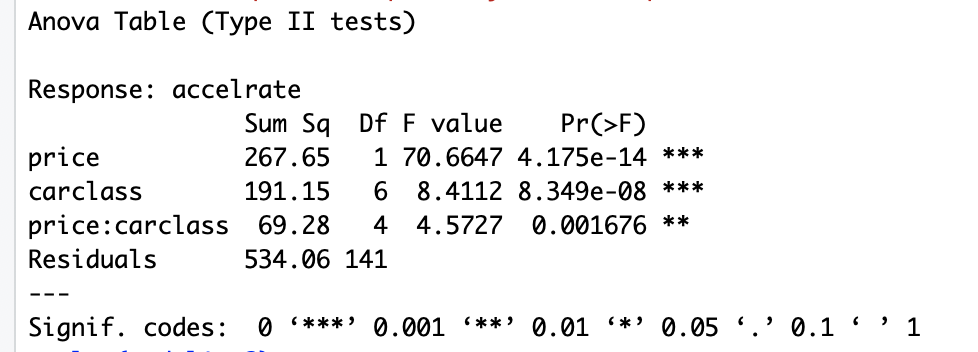
\includegraphics[width=0.95\textwidth]{../graphics/TWATable}\\
	\hline
	\end{tabular}	
	\caption{Two Way ANOVA.} %6
	\label{fig:TWATAB}
\end{table}

As with any ANOVA, we must meet the required assumptions of normal distribution of model residuals and homogeneity of variance of the groups. For the first assumption, normal distribution of model residuals, we generated a qq plot of the model residuals as seen in Figure~\ref{fig:TWAQQ}. As can be seen in this figure, there is not an apparent departure from normality so we accept that this assumption holds. The second assumption also holds as seen in Figure~\ref{fig:TWARES} since the plot shows a random cloud that supports homogeneity of variance. As a validation of these assumptions a Shapiro-Wilk normality test and Levene's Test for Homogeneity of Variance were also performed which support these assumption are met. Table~\ref{fig:TWAASS} shows these results. While the p-value of the Shapiro-Wilk normality test is inconclusive for normality, the QQ plot in Figure~\ref{fig:TWAQQ} gives us confidence of normality.
\begin{table}[h]
\centering
\begin{tabular}{p{0.48\textwidth} p{0.48\textwidth}}
	\hline
	\multicolumn{1}{|c|}{Normality} & \multicolumn{1}{|c|}{Equal Variance} \\
		\multicolumn{1}{|c|}{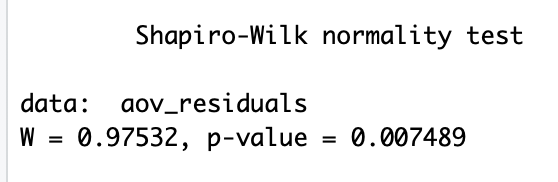
\includegraphics[width=0.48\textwidth]{../graphics/TWAshap}} &
		\multicolumn{1}{|c|}{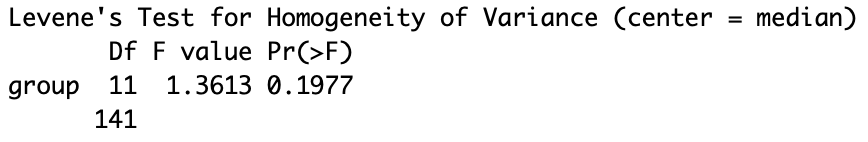
\includegraphics[width=0.48\textwidth]{../graphics/TWALev}}\\
		\hline
	\end{tabular}		
	\caption{Two Way ANOVA Assumptions.} %6
	\label{fig:TWAASS}
\end{table}
 Since we do have a significant interaction effect, we want to look at all the separate group combinations. Figure~\ref{fig:PHT} shows the results from this analysis. Table~\ref{fig:TWALS} shows a summary of the lsmeans between each \texttt{carclass} and each \texttt{price} combination. 
 \begin{table}[h]
\centering
\begin{tabular}{p{0.45\textwidth}}
	\hline
	\multicolumn{1}{|c|}{}\\
		\multicolumn{1}{|c|}{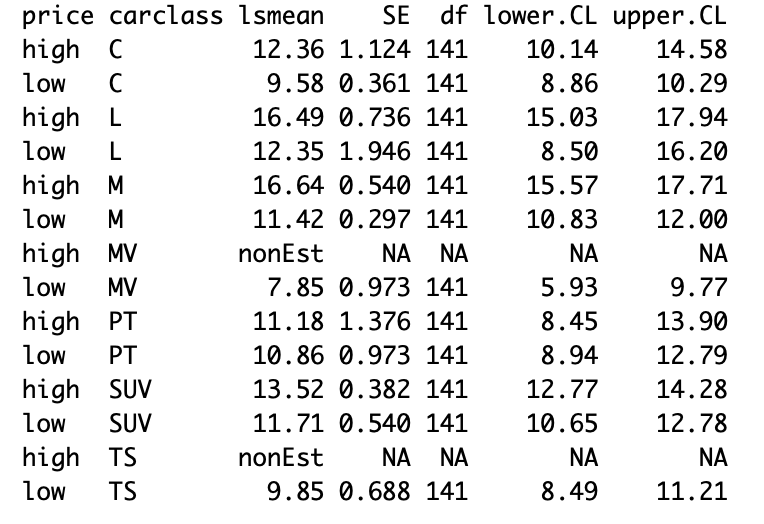
\includegraphics[width=0.45\textwidth]{../graphics/TWAls}}\\
		\hline
	\end{tabular}		
	\caption{Posthoc Analysis of Interactions.} %6
	\label{fig:TWALS}
\end{table}
\subsection{Conclusion/Discussion}
Using the Two-Way ANOVA, we can look at the separate group combinations between \texttt{price} and \texttt{carclass}. Looking at Table~\ref{fig:PHT} we can see which combinations of interactions are statistically significant. Using a 95\% confidence interval and applying a tukey adjustment for comparing the family of 14 estimates we see that the following statistically significant interpretations can be made:\\
\begin{itemize}
\item[] \textbf{low, C - high, L} Holding all things constant, a HEV in \texttt{carclass} C with a \texttt{price} less than \$40,000 will have an acceleration rate 6.9 seconds slower than a HEV in \texttt{carclass} L with a \texttt{price} greater than \$40,000. So a large HEV with an msrp greater than \$40,000 will reach 60 miles per hour 6.9 seconds faster than a compact HEV with a msrp less than \$40,000.
\item[] \textbf{low, C - high, M} Holding all things constant, a HEV in \texttt{carclass} C with a \texttt{price} less than \$40,000 will have an acceleration rate 7.0 seconds slower than a HEV in \texttt{carclass} M with a \texttt{price} greater than \$40,000. So a midsize HEV with an msrp greater than \$40,000 will reach 60 miles per hour 7.0 seconds faster than a compact HEV with a msrp less than \$40,000.
\item[] \textbf{low, C - high, SUV} Holding all things constant, a HEV in \texttt{carclass} C with a \texttt{price} less than \$40,000 will have an acceleration rate 3.9 seconds slower than a HEV in \texttt{carclass} SUV with a \texttt{price} greater than \$40,000. So a sport utility HEV with an msrp greater than \$40,000 will reach 60 miles per hour 3.9 seconds faster than a compact HEV with a msrp less than \$40,000.
\item[] \textbf{high, L - low, M} Holding all things constant, a HEV in \texttt{carclass} L with a \texttt{price} greater than \$40,000 will have an acceleration rate 5.1 seconds faster than a HEV in \texttt{carclass} M with a \texttt{price} less than \$40,000. So a large HEV with an msrp greater than \$40,000 will reach 60 miles per hour 5.1 seconds faster than a midsize HEV with a msrp less than \$40,000.
\item[] \textbf{high, L - low, MV} Holding all things constant, a HEV in \texttt{carclass} L with a \texttt{price} greater than \$40,000 will have an acceleration rate 8.6 seconds faster than a HEV in \texttt{carclass} MV with a \texttt{price} less than \$40,000. So a large HEV with an msrp greater than \$40,000 will reach 60 miles per hour 5.1 seconds faster than a mini van HEV with a msrp less than \$40,000.
\item[] \textbf{high, L - low, TS} Holding all things constant, a HEV in \texttt{carclass} L with a \texttt{price} greater than \$40,000 will have an acceleration rate 6.6 seconds faster than a HEV in \texttt{carclass} TS with a \texttt{price} less than \$40,000. So a large HEV with an msrp greater than \$40,000 will reach 60 miles per hour 6.6 seconds faster than a two-seater HEV with a msrp less than \$40,000.
\item[] \textbf{high, M - low, M} Holding all things constant, a HEV in \texttt{carclass} M with a \texttt{price} greater than \$40,000 will have an acceleration rate 5.2 seconds faster than a HEV in \texttt{carclass} M with a \texttt{price} less than \$40,000. So a midsize HEV with an msrp greater than \$40,000 will reach 60 miles per hour 5.2 seconds faster than a midsize HEV with a msrp less than \$40,000.
\item[] \textbf{high, M - low, MV} Holding all things constant, a HEV in \texttt{carclass} M with a \texttt{price} greater than \$40,000 will have an acceleration rate 8.8 seconds faster than a HEV in \texttt{carclass} MV with a \texttt{price} less than \$40,000. So a midsize HEV with an msrp greater than \$40,000 will reach 60 miles per hour 8.8 seconds faster than a mini van HEV with a msrp less than \$40,000.
\item[] \textbf{high, M - low, SUV} Holding all things constant, a HEV in \texttt{carclass} M with a \texttt{price} greater than \$40,000 will have an acceleration rate 4.9 seconds faster than a HEV in \texttt{carclass} SUV with a \texttt{price} less than \$40,000. So a midsize HEV with an msrp greater than \$40,000 will reach 60 miles per hour 4.9 seconds faster than a sport utility HEV with a msrp less than \$40,000.
\item[] \textbf{high, M - low, TS} Holding all things constant, a HEV in \texttt{carclass} M with a \texttt{price} greater than \$40,000 will have an acceleration rate 6.8 seconds faster than a HEV in \texttt{carclass} TS with a \texttt{price} less than \$40,000. So a midsize HEV with an msrp greater than \$40,000 will reach 60 miles per hour 6.8 seconds faster than a two-seater HEV with a msrp less than \$40,000.
\item[] \textbf{low, MV - high, SUV} Holding all things constant, a HEV in \texttt{carclass} MV with a \texttt{price} less than \$40,000 will have an acceleration rate 5.7 seconds slower than a HEV in \texttt{carclass} SUV with a \texttt{price} greater than \$40,000. So a sport utility HEV with an msrp greater than \$40,000 will reach 60 miles per hour 5.7 seconds faster than a mini van HEV with a msrp less than \$40,000.
\end{itemize}

These results are very beneficial in determining which vehicle is most appropriate for the type of driving that is desired. From these results it is easy to see that if the acceleration rate is important to a consumer, then in general vehicles with an msrp greater than \$40,000 will have higher acceleration rates. It was disappointing that none of the group combinations of identical \texttt{carclass} were not statistically significant, nor were group combinations of identical \texttt{price} combinations. The two-way ANOVA provided insight into some of the factors that were not apparent in the multiple linear regression model.

\pagebreak
\appendix{} 
\section{Graphics and Summary Tables}
\begin{figure}[H] % [h] forces the figure to be output where it is defined in the code (it suppresses floating)
	\centering
	\begin{tabular}{| p{0.95\textwidth}|}
	\hline
	\\
	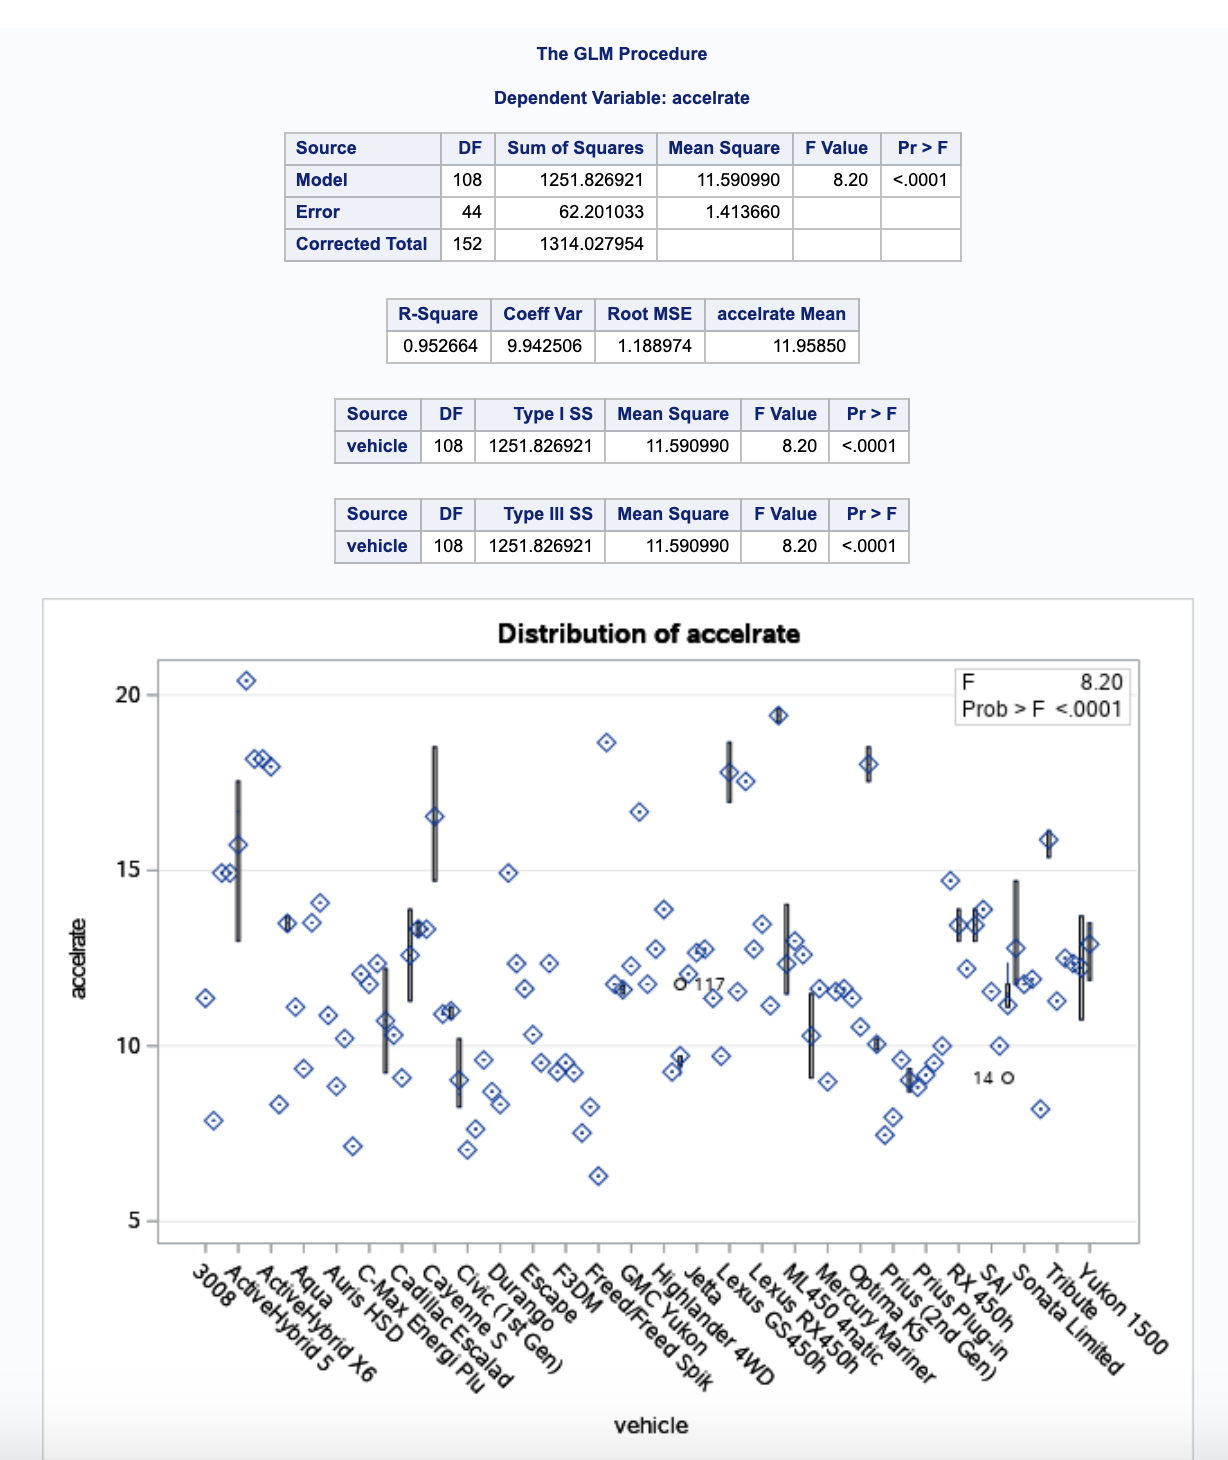
\includegraphics[width=0.95\textwidth]{../graphics/AccelrateByVehicle}\\
	\hline
	\end{tabular}	
	\caption{Accelrate by Vehicle.} %6
	\label{fig:ABV}
\end{figure}
\begin{figure}[H] % [h] forces the figure to be output where it is defined in the code (it suppresses floating)
	\centering
	\begin{tabular}{| p{0.95\textwidth}|}
	\hline
	\\
	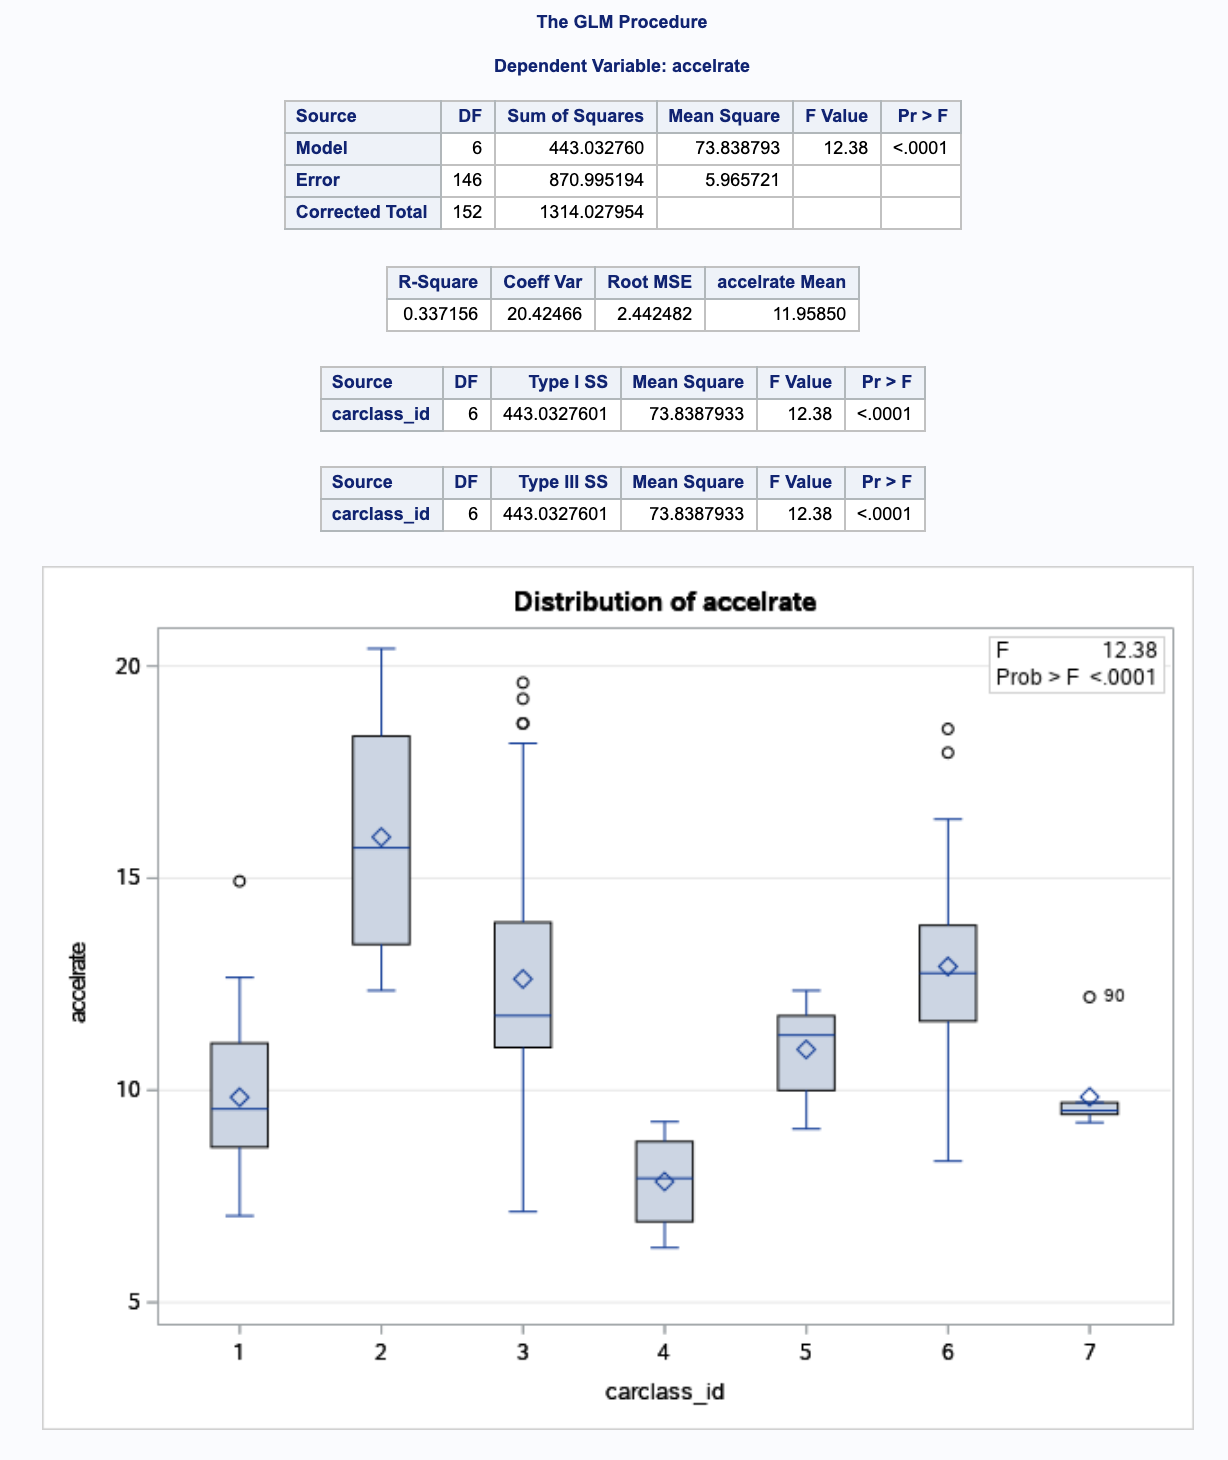
\includegraphics[width=0.95\textwidth]{../graphics/AccelrateByCarclass}\\
	\hline
	\end{tabular}	
	\caption{Accelrate by Car Class.} %6
	\label{fig:ABCC}
\end{figure}
\begin{figure}[H] % [h] forces the figure to be output where it is defined in the code (it suppresses floating)
	\centering
	\begin{tabular}{| p{0.95\textwidth}|}
	\hline
	\\
	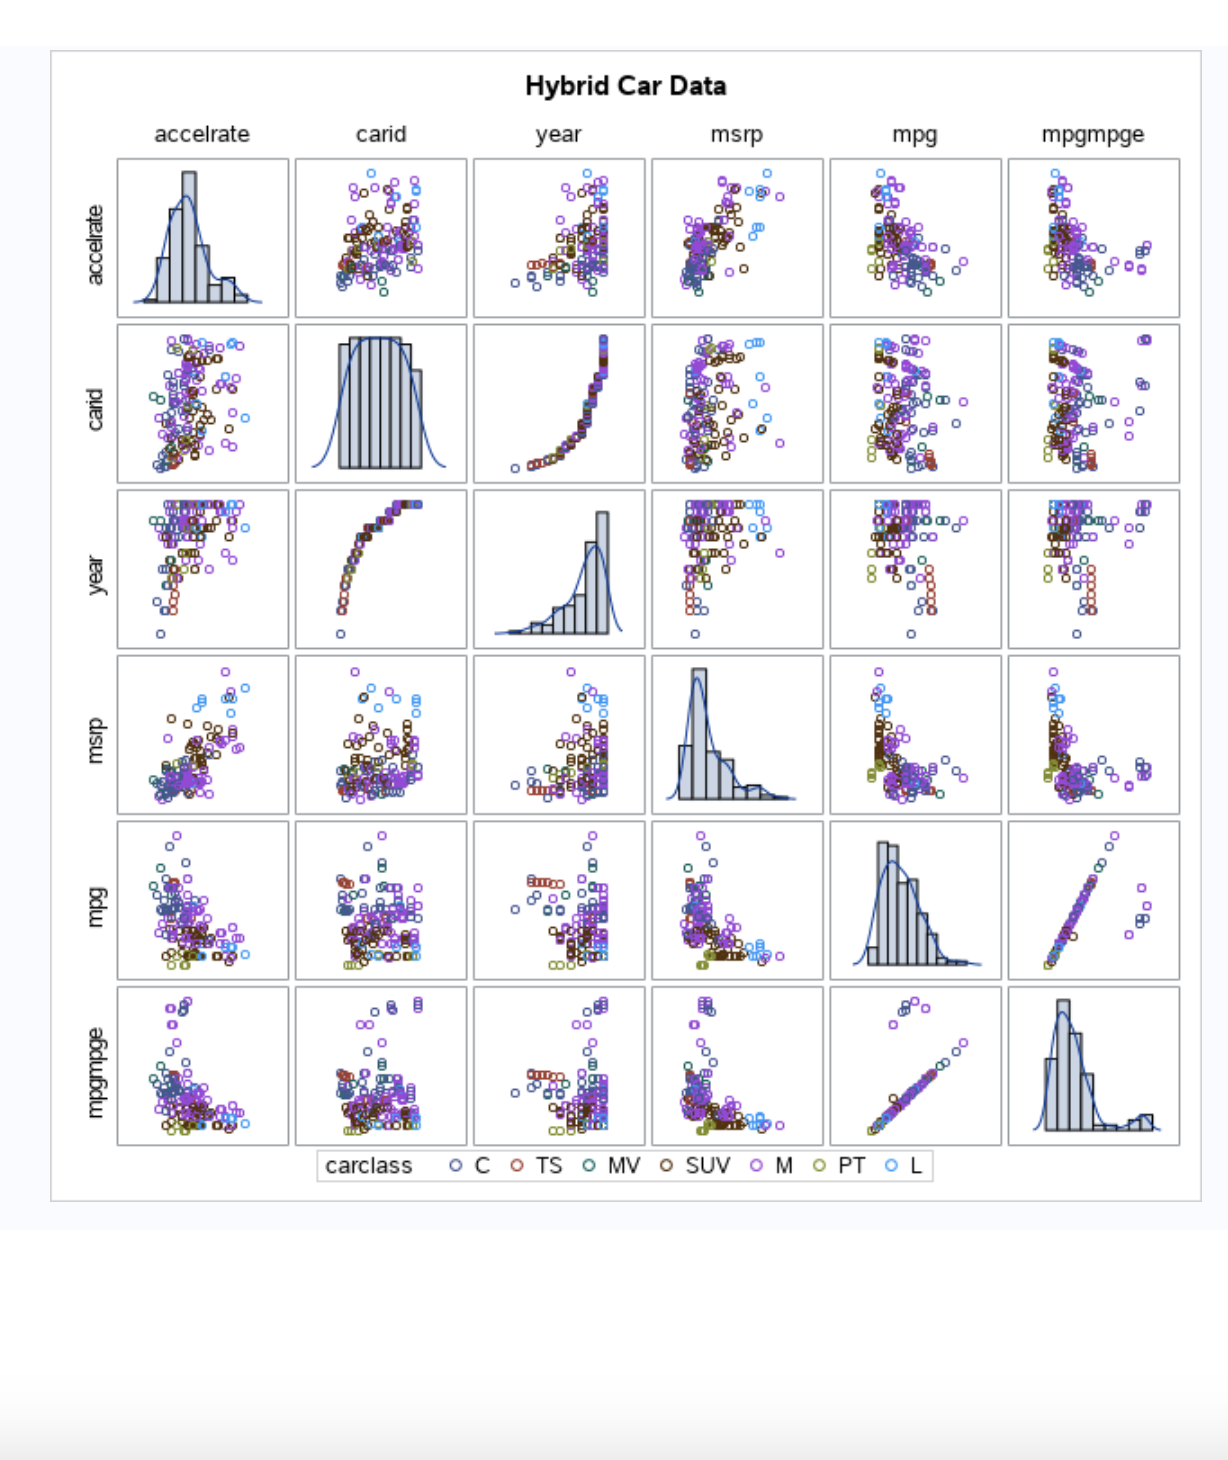
\includegraphics[width=0.95\textwidth]{../graphics/ScatterPlot}\\
	\hline
	\end{tabular}	
	\caption{Scatter Plot Matrix by Car Class.} %6
	\label{fig:SCAT}
\end{figure}

\begin{figure}[H] % [h] forces the figure to be output where it is defined in the code (it suppresses floating)
	\centering
	\begin{tabular}{p{0.48\textwidth} p{0.48\textwidth}}
	\hline
	\multicolumn{1}{|c|}{Simple Statistics} & \multicolumn{1}{|c|}{Scatter Plot Matrix} \\
		\multicolumn{1}{|c|}{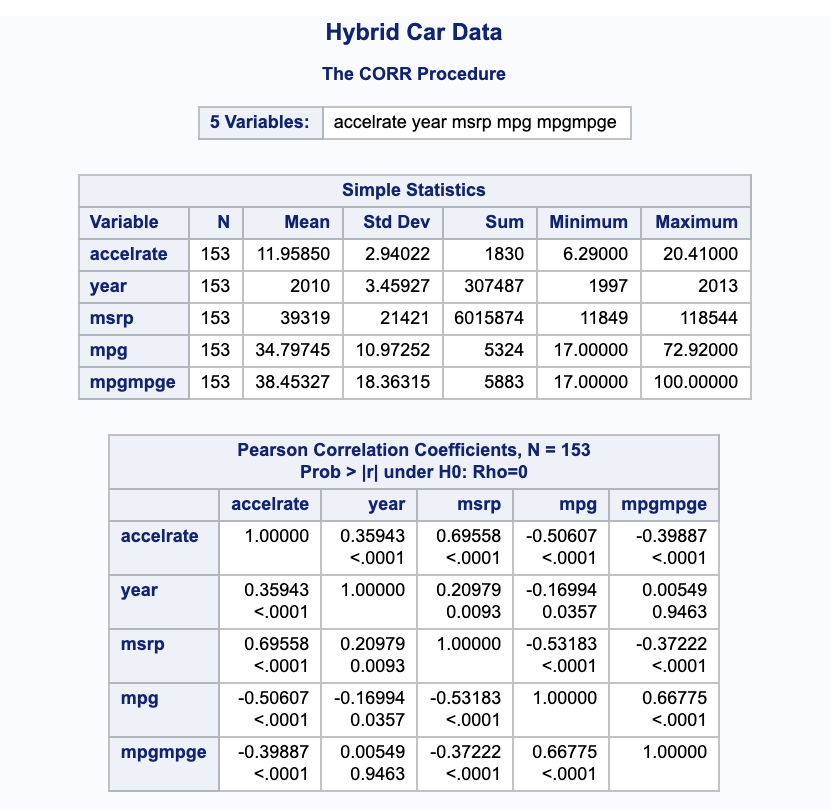
\includegraphics[width=0.48\textwidth]{../graphics/PearsonVariables1}} &
		\multicolumn{1}{|c|}{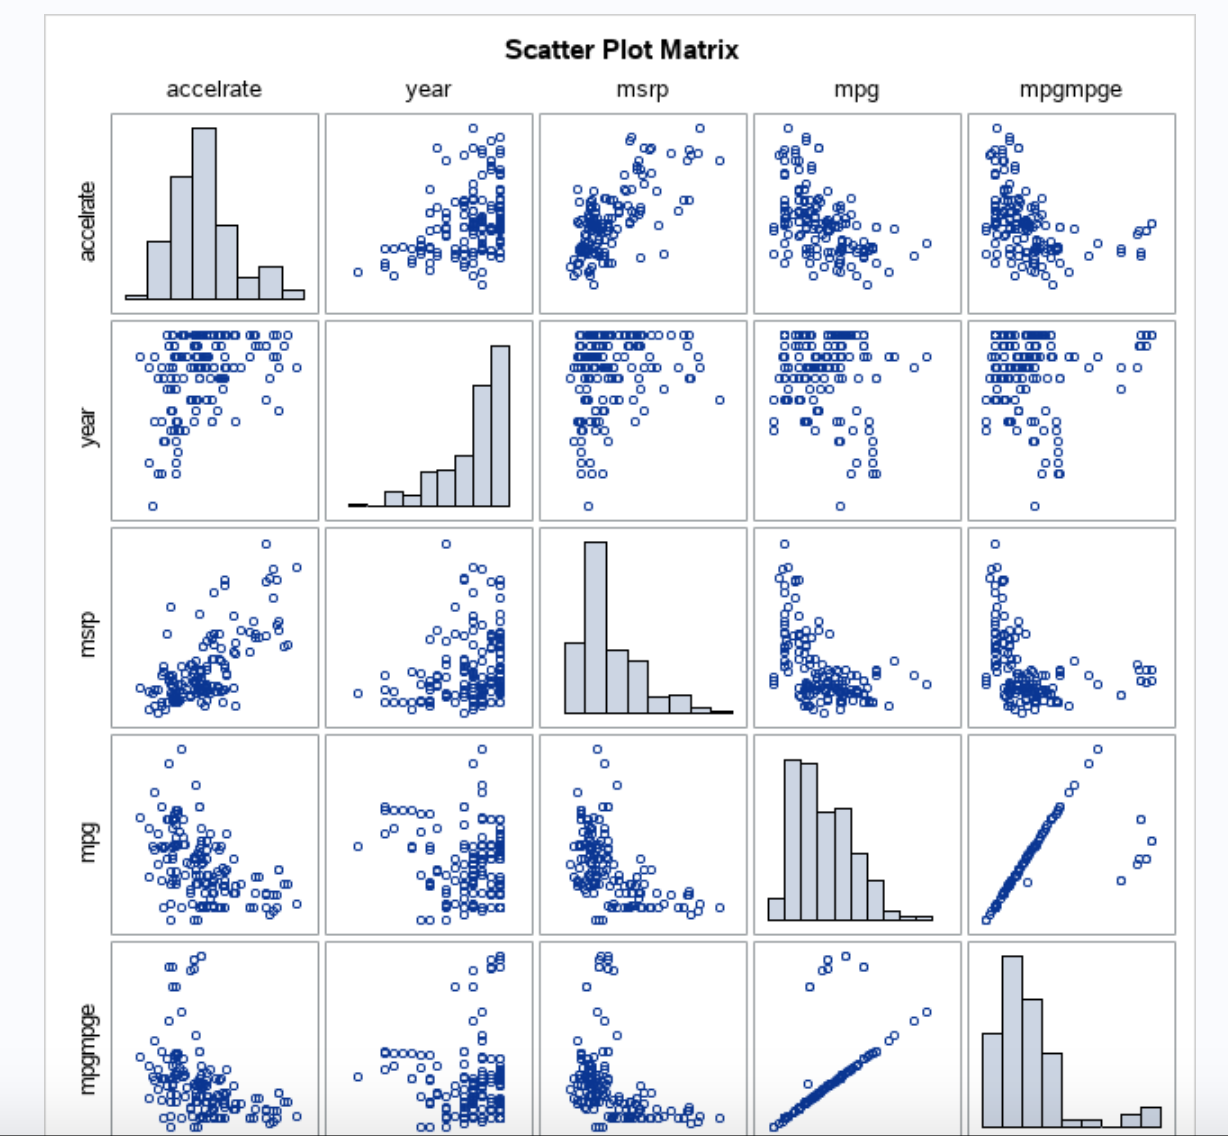
\includegraphics[width=0.48\textwidth]{../graphics/PearsonVariables2}}\\
		\hline
	\end{tabular}		
	\caption{Hybrid Car Data Correlation.} %1
	\label{fig:HCDPC}
\end{figure}

\begin{figure}[H] % [h] forces the figure to be output where it is defined in the code (it suppresses floating)
	\centering
	\begin{tabular}{p{0.48\textwidth} p{0.48\textwidth}}
	\hline
	\multicolumn{1}{|c|}{Simple Statistics} & \multicolumn{1}{|c|}{Scatter Plot Matrix} \\
		\multicolumn{1}{|c|}{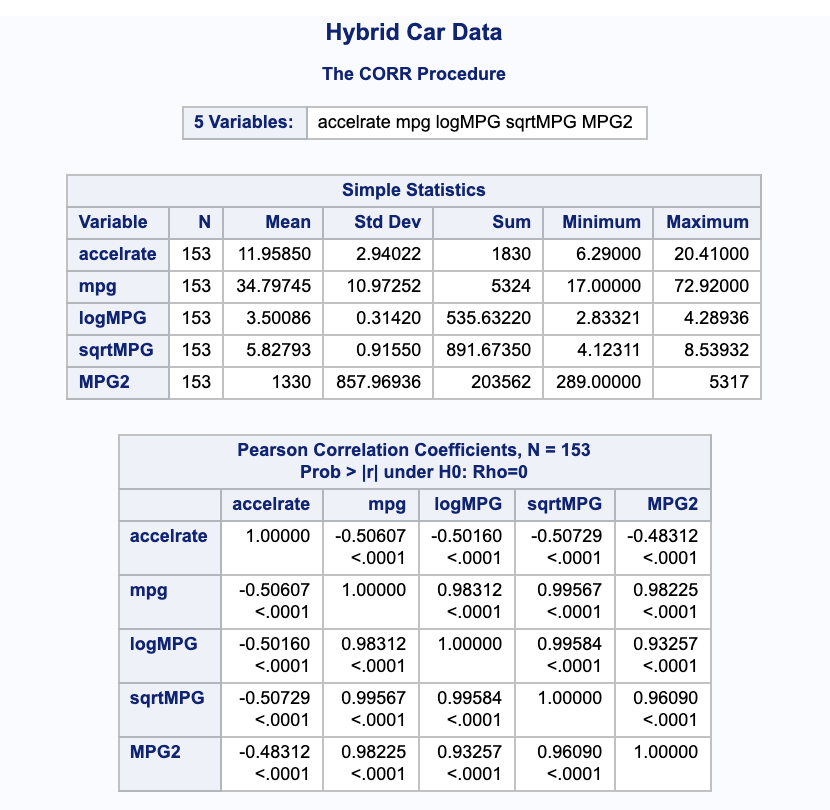
\includegraphics[width=0.48\textwidth]{../graphics/PearsonTransform1}} &
		\multicolumn{1}{|c|}{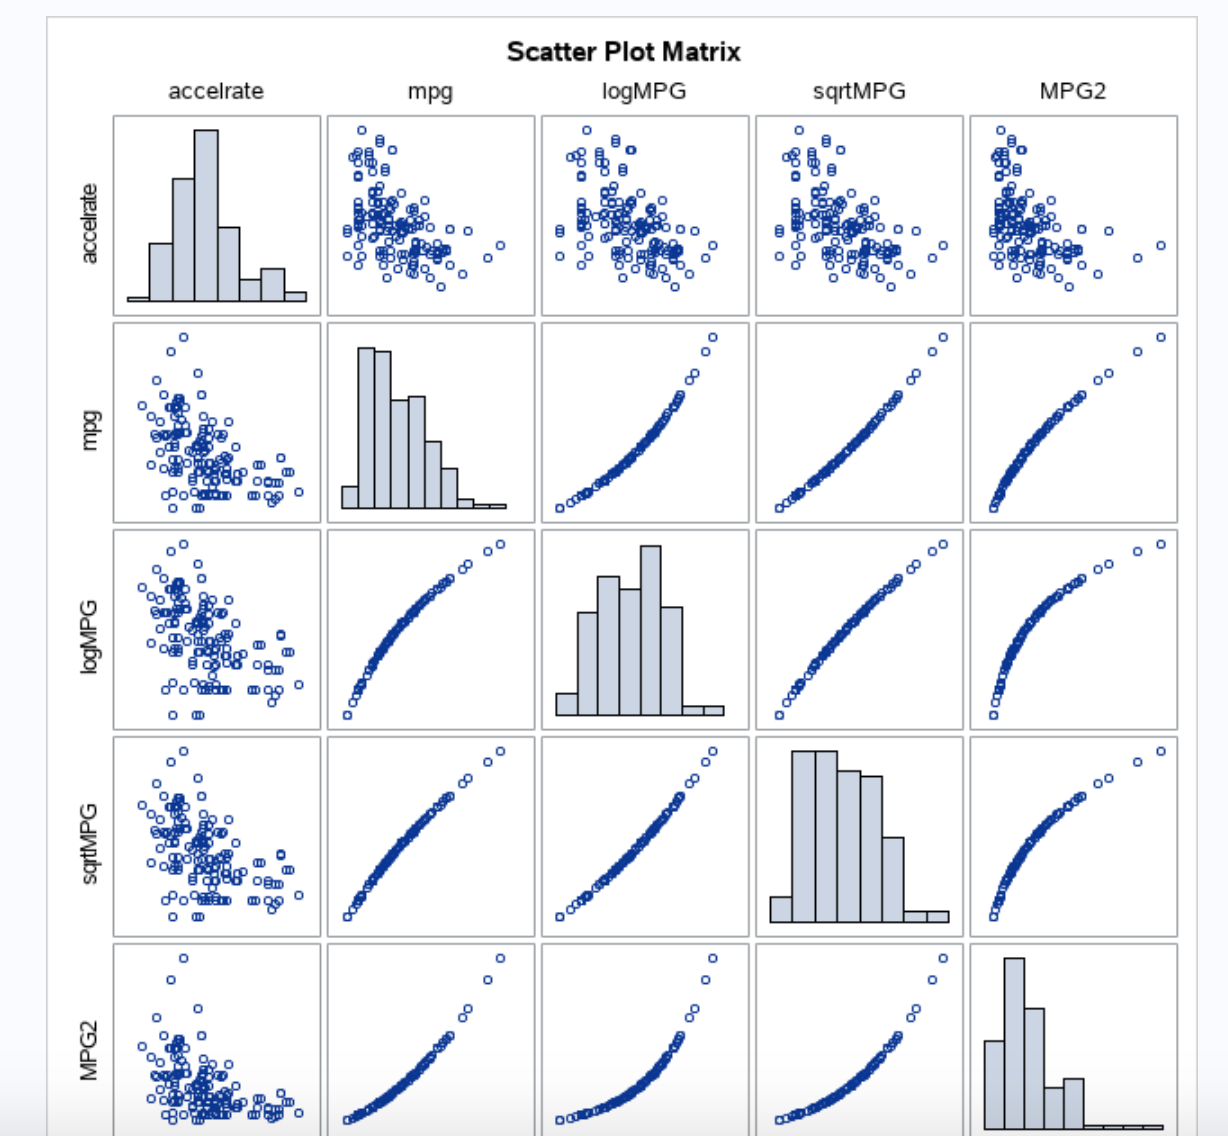
\includegraphics[width=0.48\textwidth]{../graphics/PearsonTransform2}}\\
		\hline
	\end{tabular}		
	\caption{Transformations of MPG vs accelrate.} %1
	\label{fig:TFPC}
\end{figure}

\begin{figure}[H] % [h] forces the figure to be output where it is defined in the code (it suppresses floating)
	\centering
	\begin{tabular}{p{0.48\textwidth} p{0.48\textwidth}}
	\hline
	\multicolumn{1}{|c|}{Simple Statistics} & \multicolumn{1}{|c|}{Scatter Plot Matrix} \\
		\multicolumn{1}{|c|}{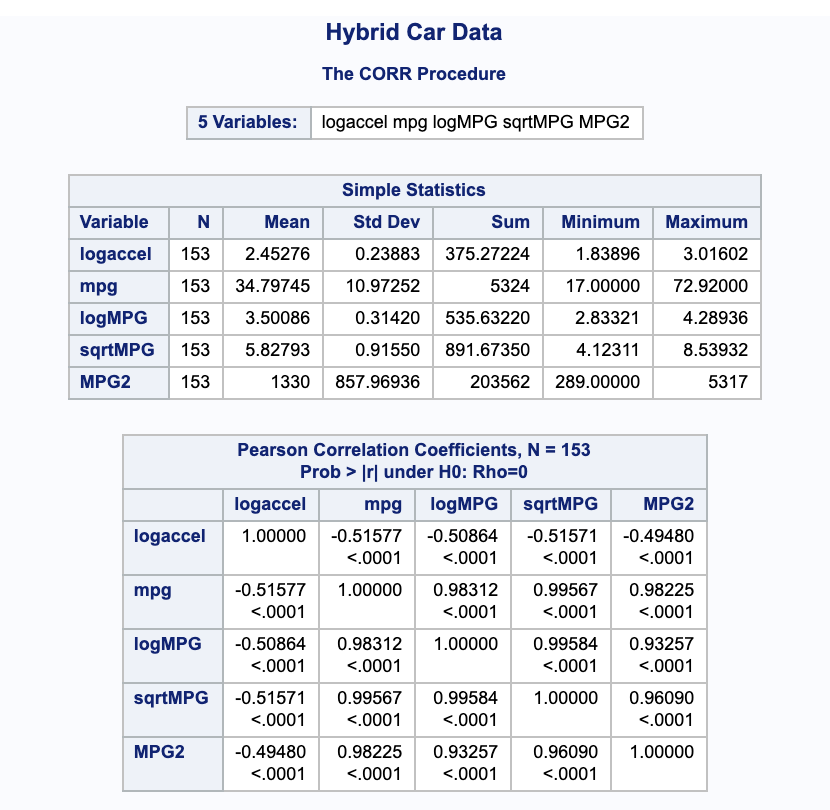
\includegraphics[width=0.48\textwidth]{../graphics/Pearsonlogacc1}} &
		\multicolumn{1}{|c|}{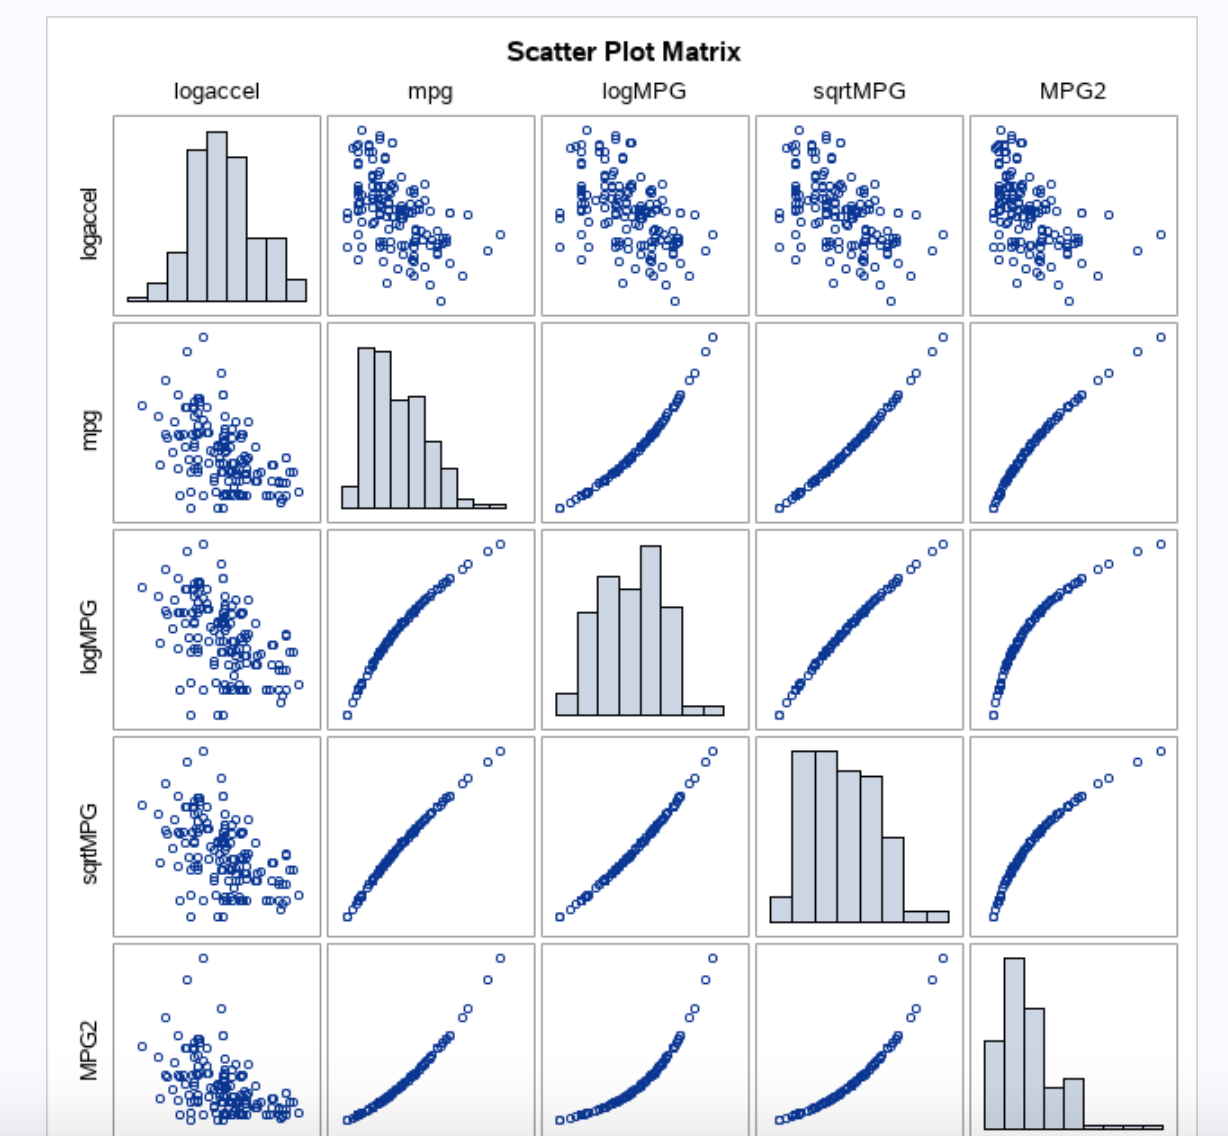
\includegraphics[width=0.48\textwidth]{../graphics/Pearsonlogacc2}}\\
		\hline
	\end{tabular}		
	\caption{Transformations of MPG vs logaccelrate.} %1
	\label{fig:TFLAPC}
\end{figure}

\begin{figure}[H] % [h] forces the figure to be output where it is defined in the code (it suppresses floating)
	\centering
	\begin{tabular}{p{0.48\textwidth} p{0.48\textwidth}}
	\hline
	\multicolumn{1}{|c|}{No Interaction} & \multicolumn{1}{|c|}{With Interaction} \\
		\multicolumn{1}{|c|}{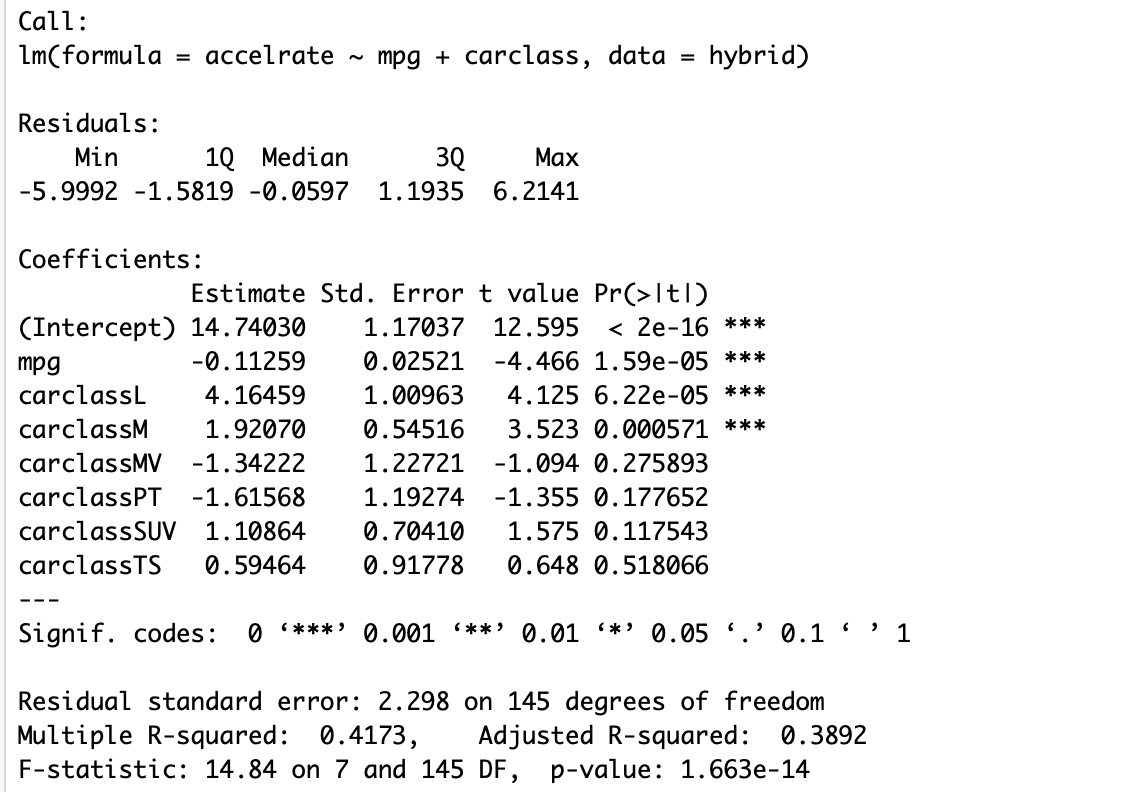
\includegraphics[width=0.48\textwidth]{../graphics/ModAccMpgNoInt}} &
		\multicolumn{1}{|c|}{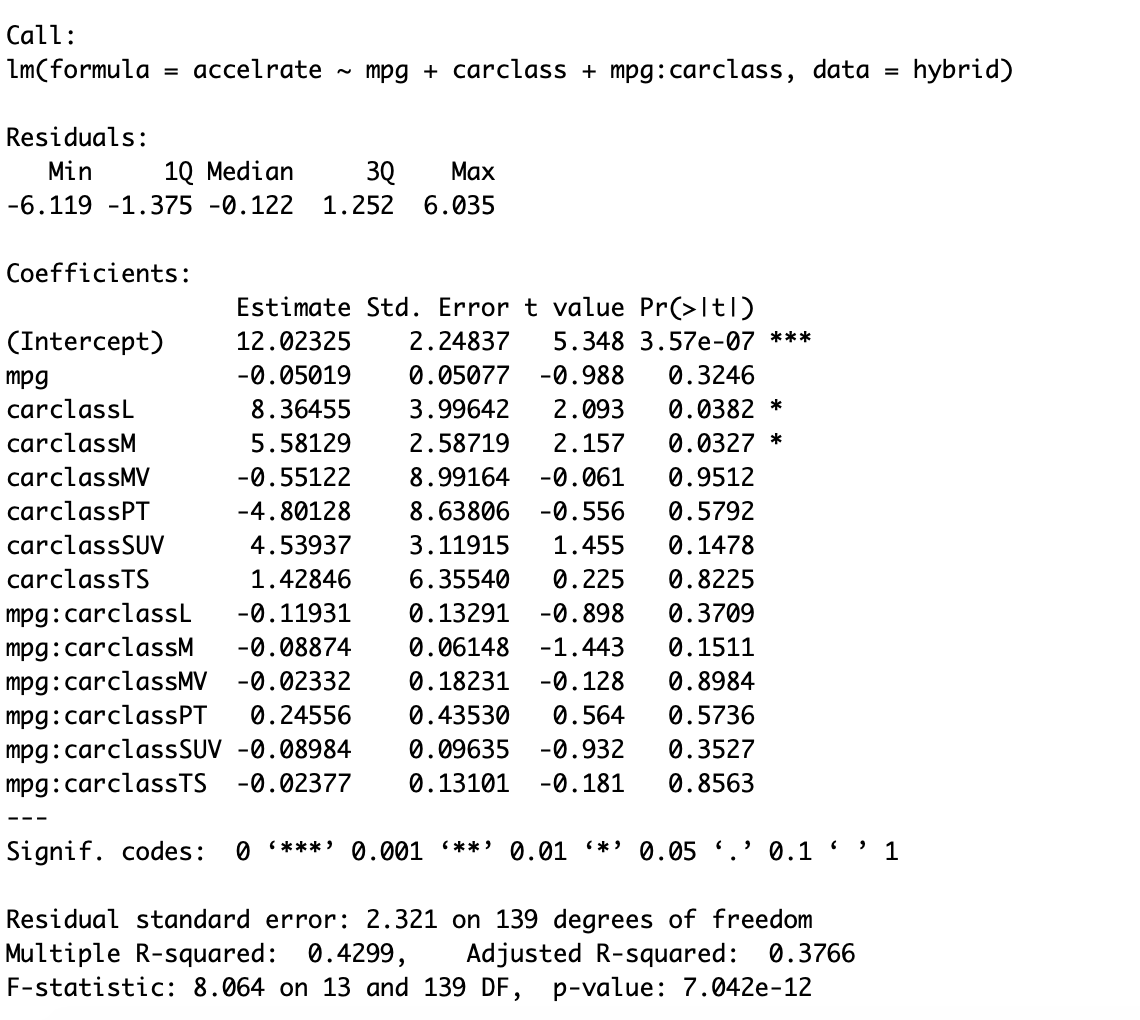
\includegraphics[width=0.48\textwidth]{../graphics/ModAccMpgInt}}\\
		\hline
		\hline
		\multicolumn{1}{|c|}{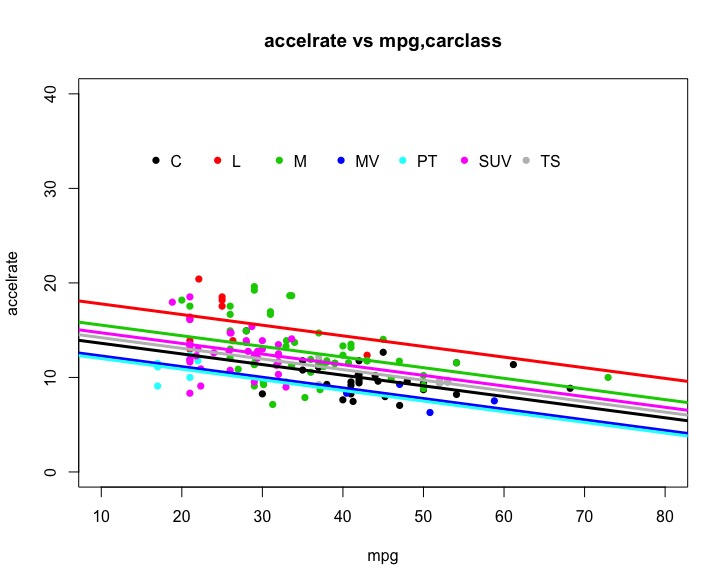
\includegraphics[width=0.48\textwidth]{../graphics/AccMpgNoInt}} &
		\multicolumn{1}{|c|}{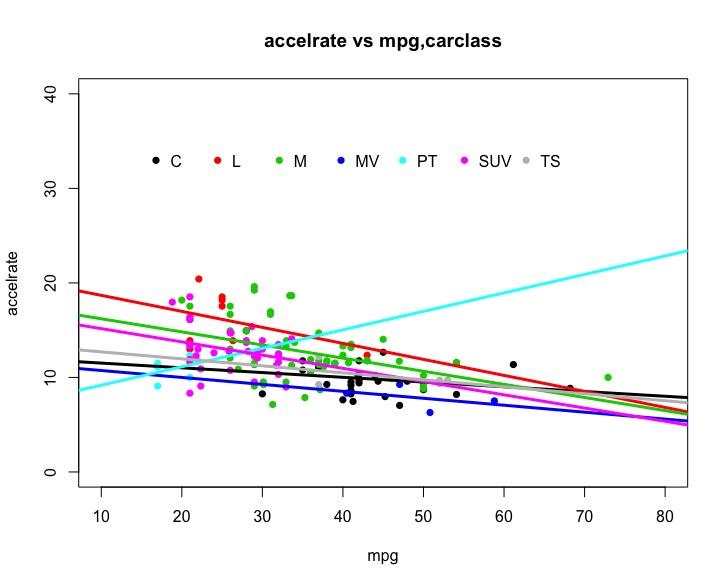
\includegraphics[width=0.48\textwidth]{../graphics/AccMpgInt}}\\
		\hline
	\end{tabular}	
	\caption{Interactions between MPG and Car Class on Accelrate.} %1
	\label{fig:INTMPG}
\end{figure}

\begin{figure}[H] % [h] forces the figure to be output where it is defined in the code (it suppresses floating)
	\centering
	\begin{tabular}{p{0.48\textwidth} p{0.48\textwidth}}
	\hline
	\multicolumn{1}{|c|}{No Interaction} & \multicolumn{1}{|c|}{With Interaction} \\
		\multicolumn{1}{|c|}{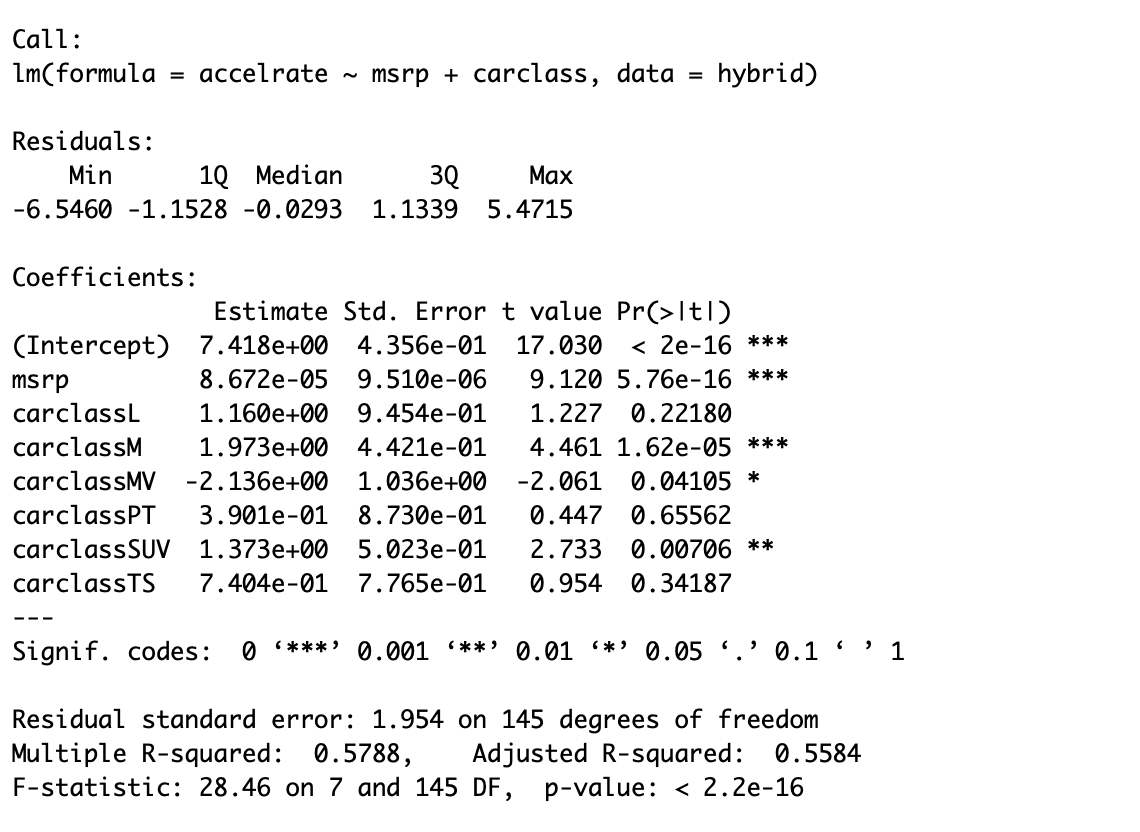
\includegraphics[width=0.48\textwidth]{../graphics/ModAccMsrpNoInt}} &
		\multicolumn{1}{|c|}{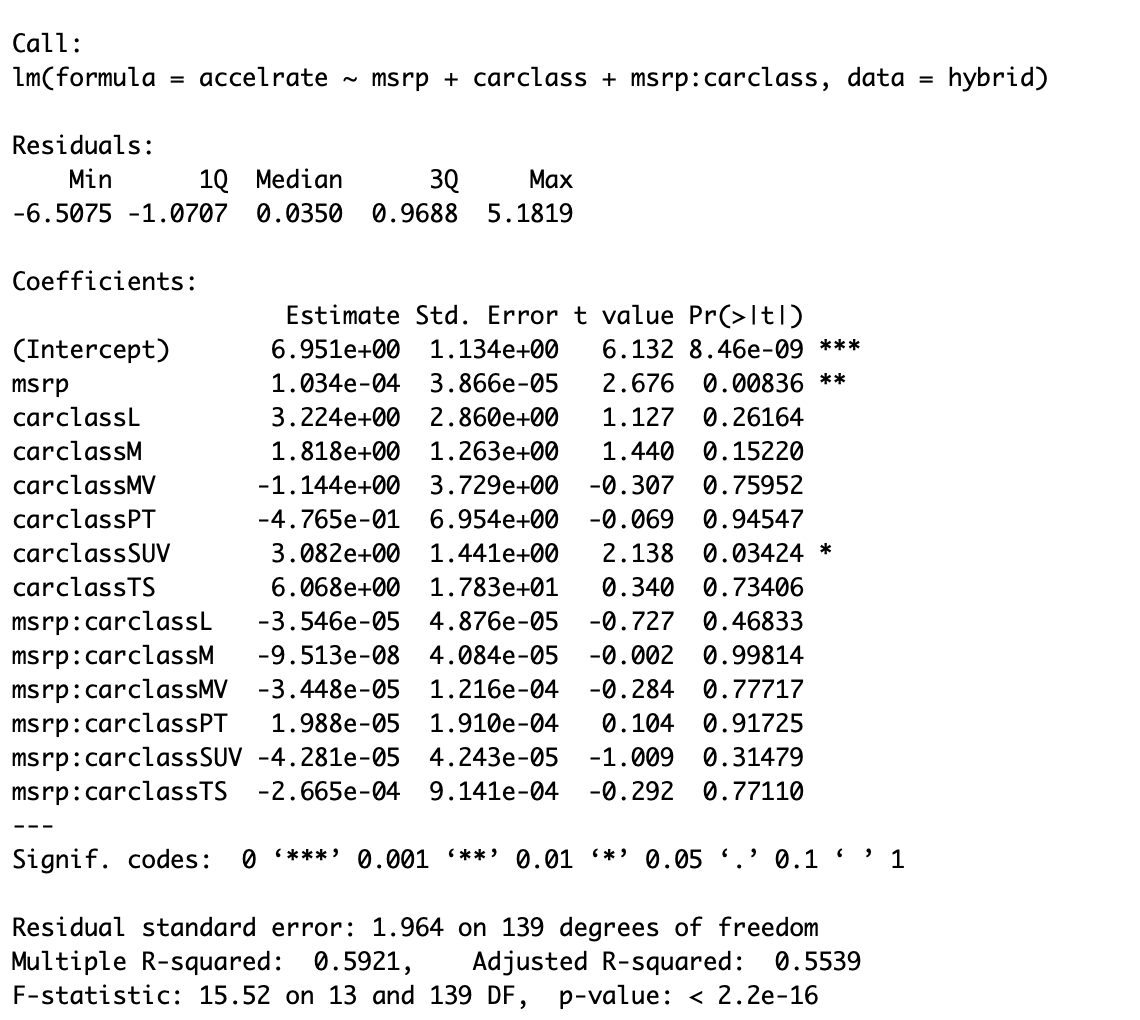
\includegraphics[width=0.48\textwidth]{../graphics/ModAccMsrpInt}}\\
		\hline
		\hline
		\multicolumn{1}{|c|}{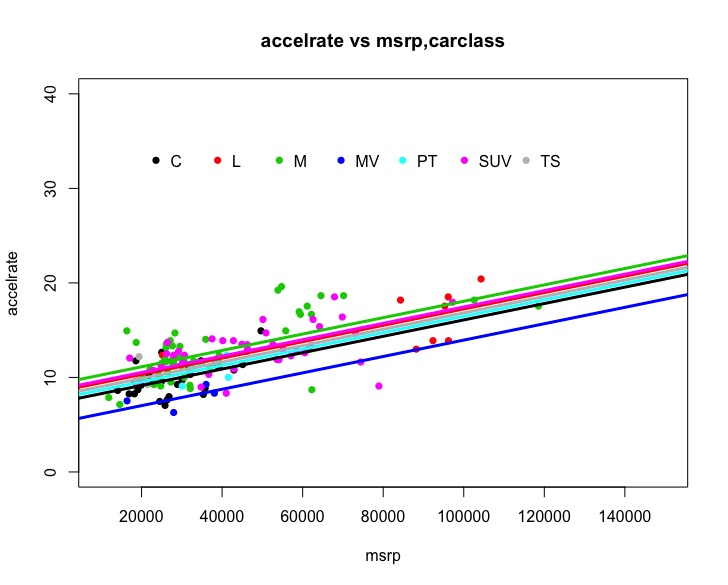
\includegraphics[width=0.48\textwidth]{../graphics/AccMsrpNoInt}} &
		\multicolumn{1}{|c|}{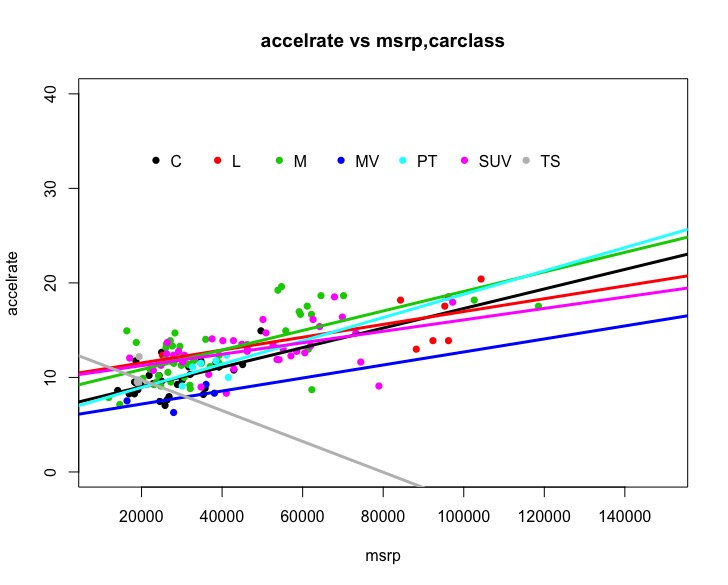
\includegraphics[width=0.48\textwidth]{../graphics/AccMsrpInt}}\\
		\hline
	\end{tabular}	
	\caption{Interactions between MSPR and Car Class on Accelrate.} %1
	\label{fig:INTMSRP}
\end{figure}

\begin{figure}[H] % [h] forces the figure to be output where it is defined in the code (it suppresses floating)
	\centering
	\begin{tabular}{p{0.48\textwidth} p{0.48\textwidth}}
	\hline
	\multicolumn{1}{|c|}{Fit Diagnostics} & \multicolumn{1}{|c|}{Residual Plots} \\
		\multicolumn{1}{|c|}{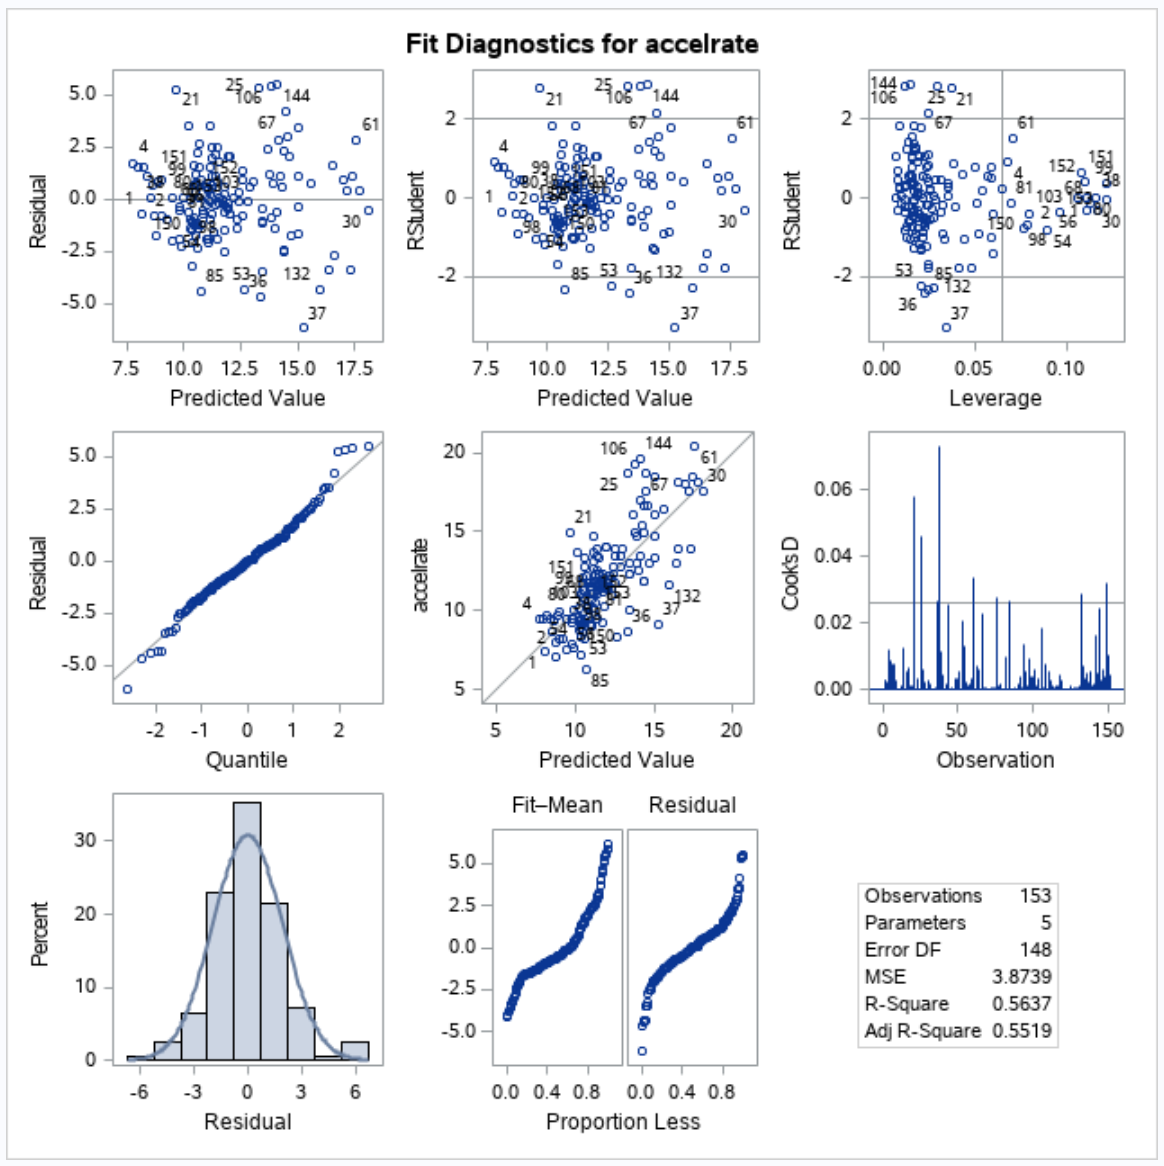
\includegraphics[width=0.48\textwidth]{../graphics/Assumptions1}} &
		\multicolumn{1}{|c|}{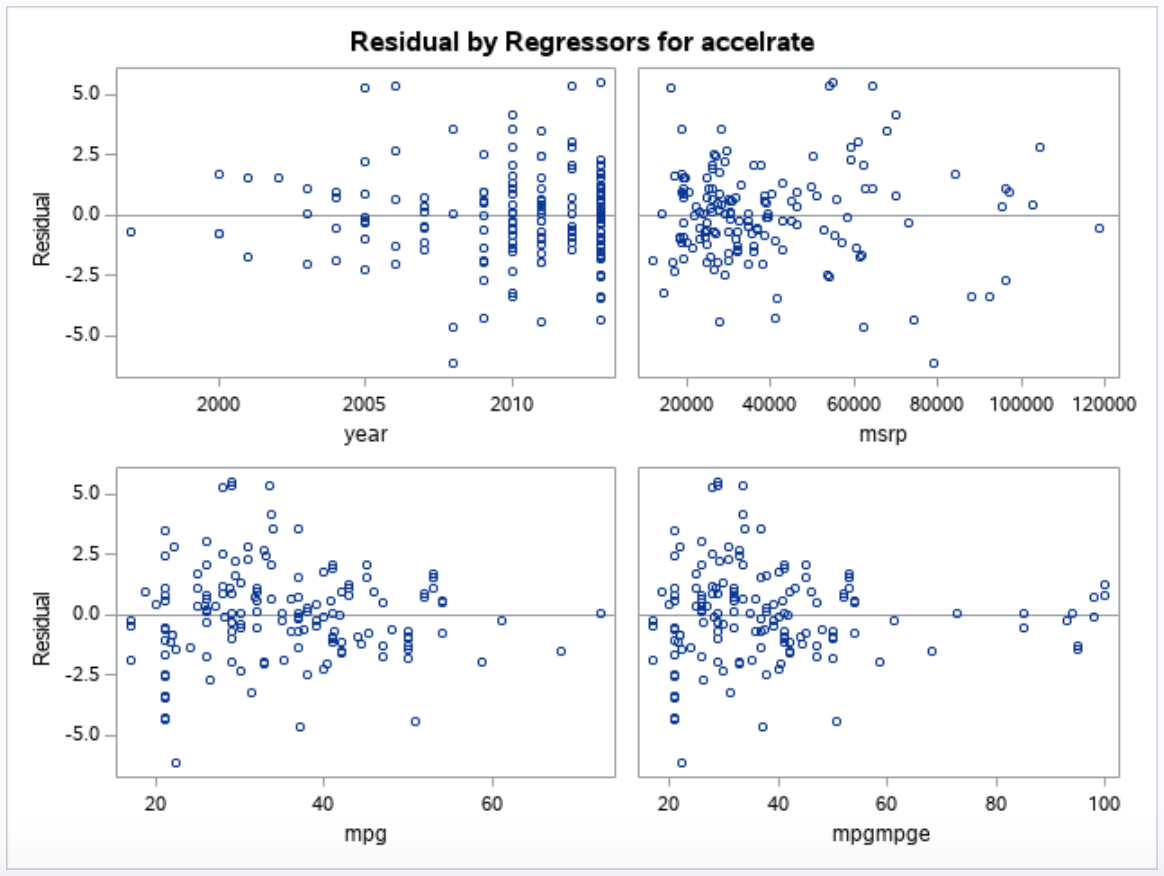
\includegraphics[width=0.48\textwidth]{../graphics/Assumptions2}}\\
		\hline
	\end{tabular}		
	\caption{Assumption Diagnostics for Hybrid Dataset.} %1
	\label{fig:ASS}
\end{figure}

\begin{figure}[H] % [h] forces the figure to be output where it is defined in the code (it suppresses floating)
	\centering
	\begin{tabular}{| p{0.95\textwidth}|}
	\hline
	\\
	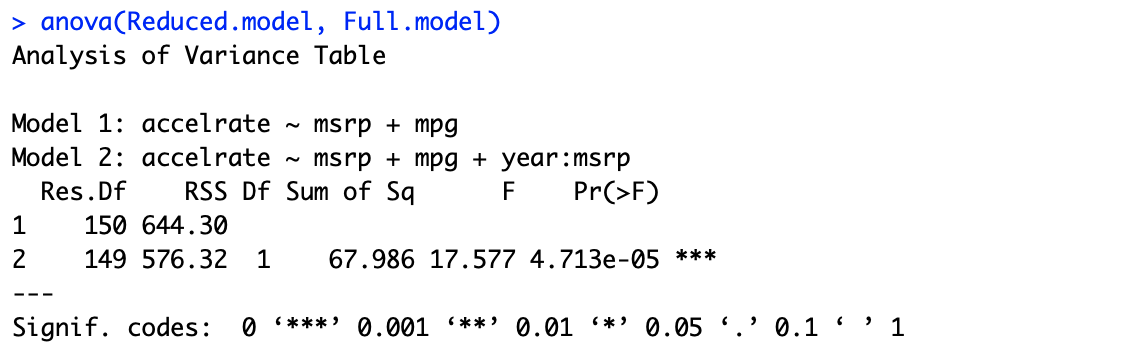
\includegraphics[width=0.95\textwidth]{../graphics/PartialFTest}\\
	\hline
	\end{tabular}	
	\caption{Partial F-Test for Final Model.} %6
	\label{fig:PFT}
\end{figure}

\begin{figure}[H] % [h] forces the figure to be output where it is defined in the code (it suppresses floating)
	\centering
	\begin{tabular}{| p{0.95\textwidth}|}
	\hline
	\\
	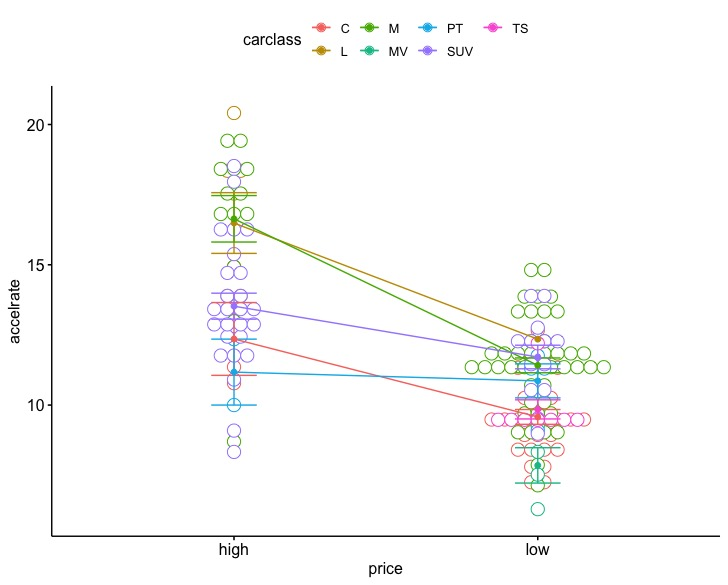
\includegraphics[width=0.95\textwidth]{../graphics/TwoWayPlot}\\
	\hline
	\end{tabular}	
	\caption{Plot of Accelrate vs Price by Car Class.} %6
	\label{fig:TWA}
\end{figure}

\begin{figure}[H] % [h] forces the figure to be output where it is defined in the code (it suppresses floating)
	\centering
	\begin{tabular}{| p{0.95\textwidth}|}
	\hline
	\\
	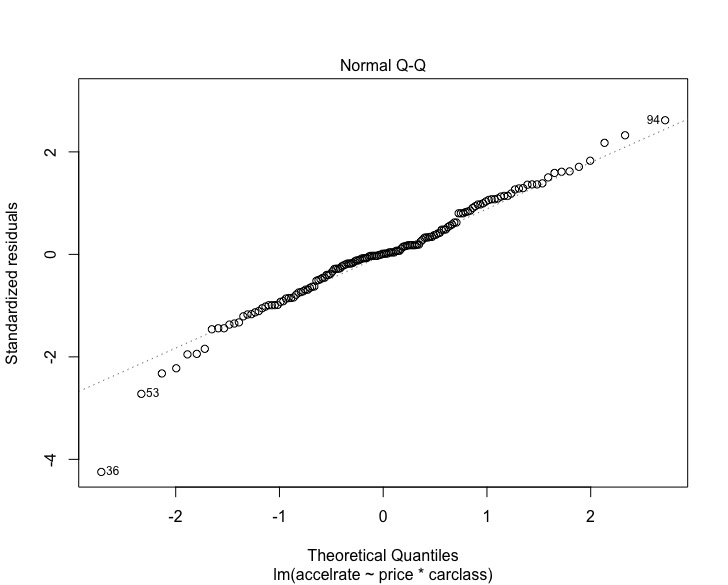
\includegraphics[width=0.95\textwidth]{../graphics/TWAqq}\\
	\hline
	\end{tabular}	
	\caption{QQ Plot of Model Residuals.} %6
	\label{fig:TWAQQ}
\end{figure}

\begin{figure}[H] % [h] forces the figure to be output where it is defined in the code (it suppresses floating)
	\centering
	\begin{tabular}{| p{0.95\textwidth}|}
	\hline
	\\
	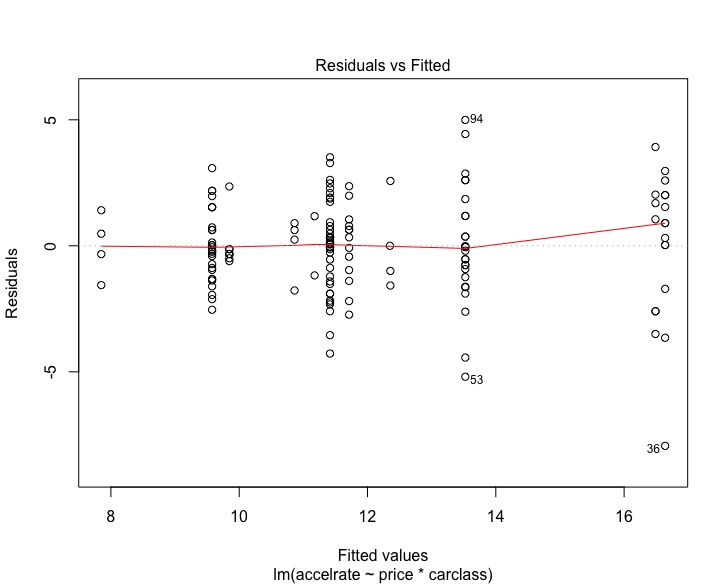
\includegraphics[width=0.95\textwidth]{../graphics/TWAresid}\\
	\hline
	\end{tabular}	
	\caption{Fitted Model Residuals.} %6
	\label{fig:TWARES}
\end{figure}

\begin{figure}[H] % [h] forces the figure to be output where it is defined in the code (it suppresses floating)
	\centering
	\begin{tabular}{p{0.48\textwidth}}
	\hline
	\multicolumn{1}{|c|}{}\\
		\multicolumn{1}{|c|}{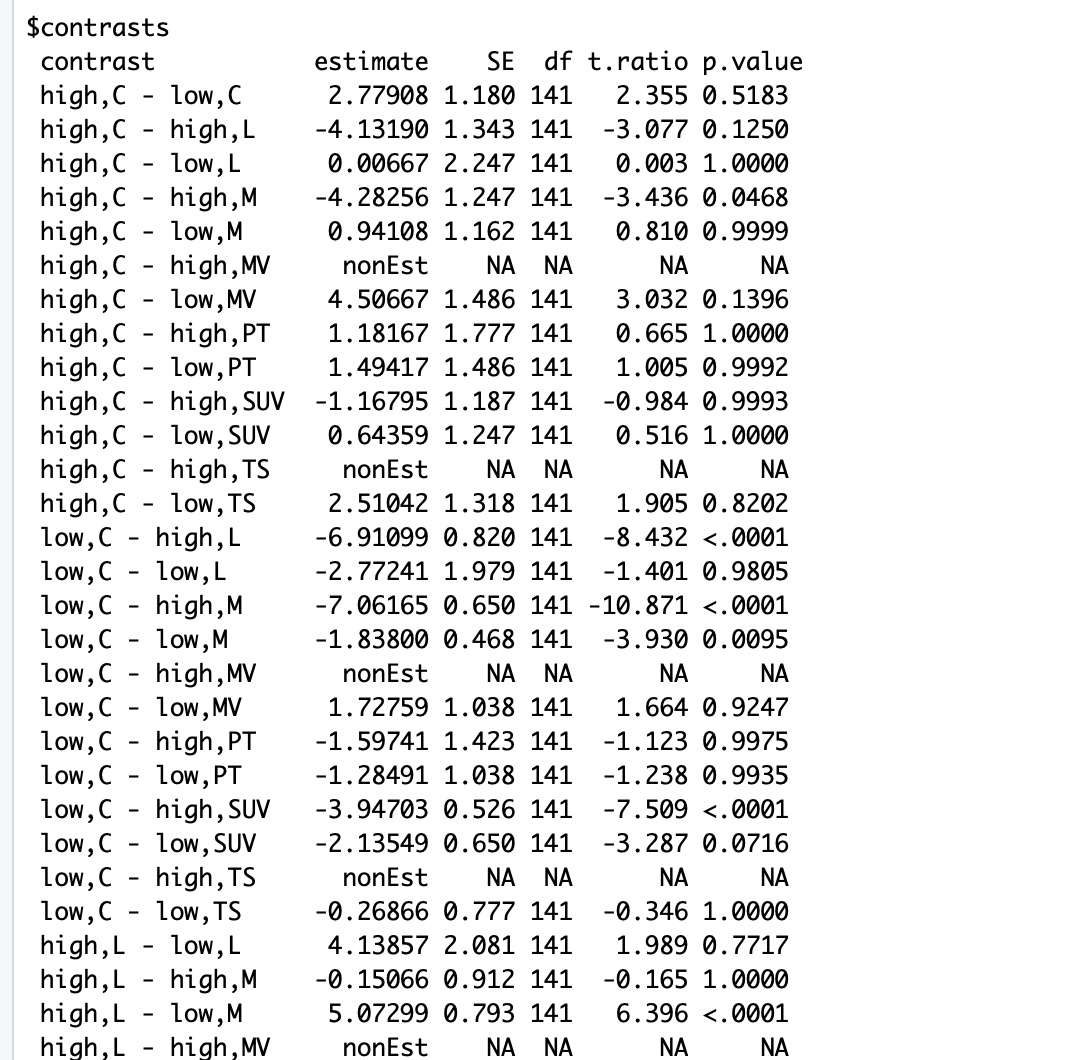
\includegraphics[width=0.48\textwidth]{../graphics/TWAcon1}}\\
		\multicolumn{1}{|c|}{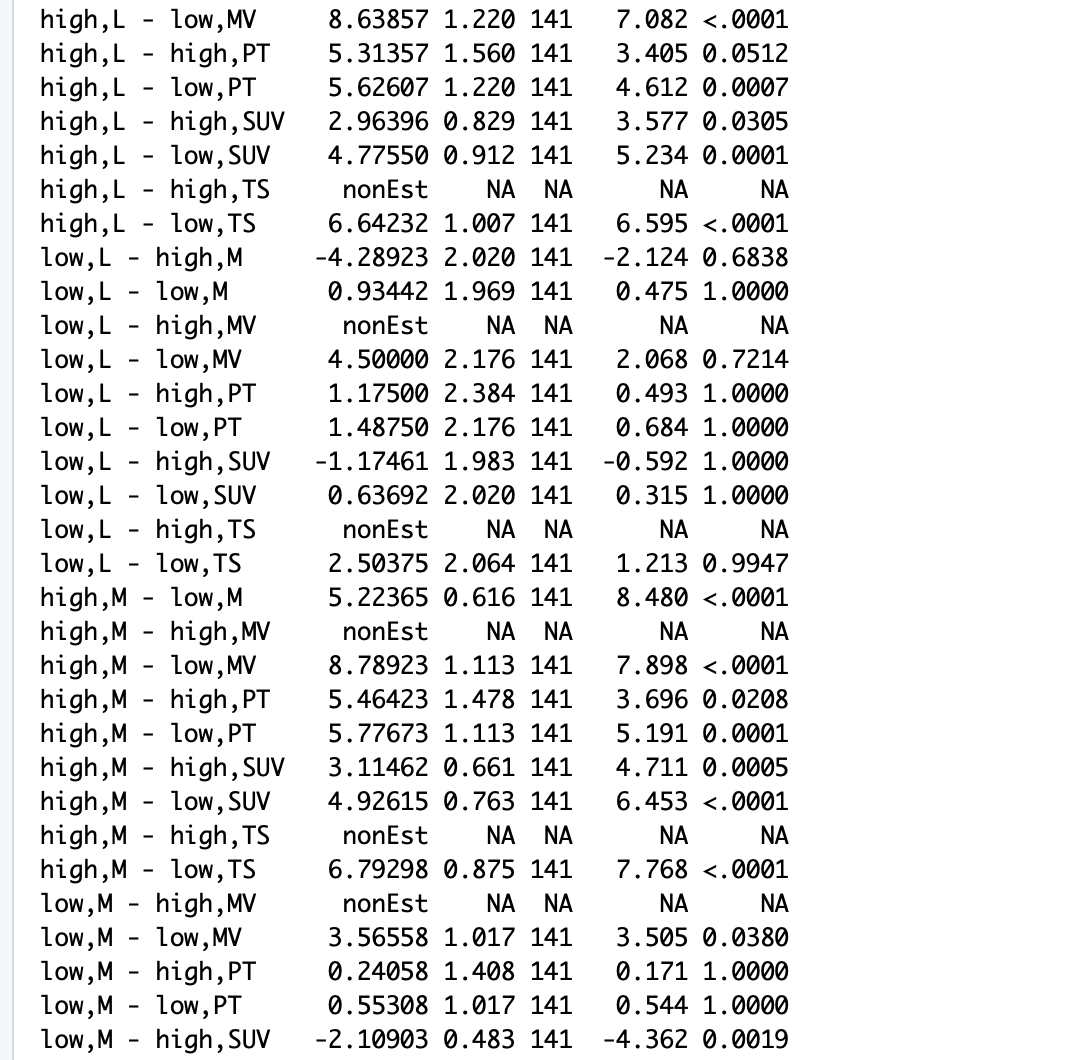
\includegraphics[width=0.48\textwidth]{../graphics/TWAcon2}}\\
		\multicolumn{1}{|c|}{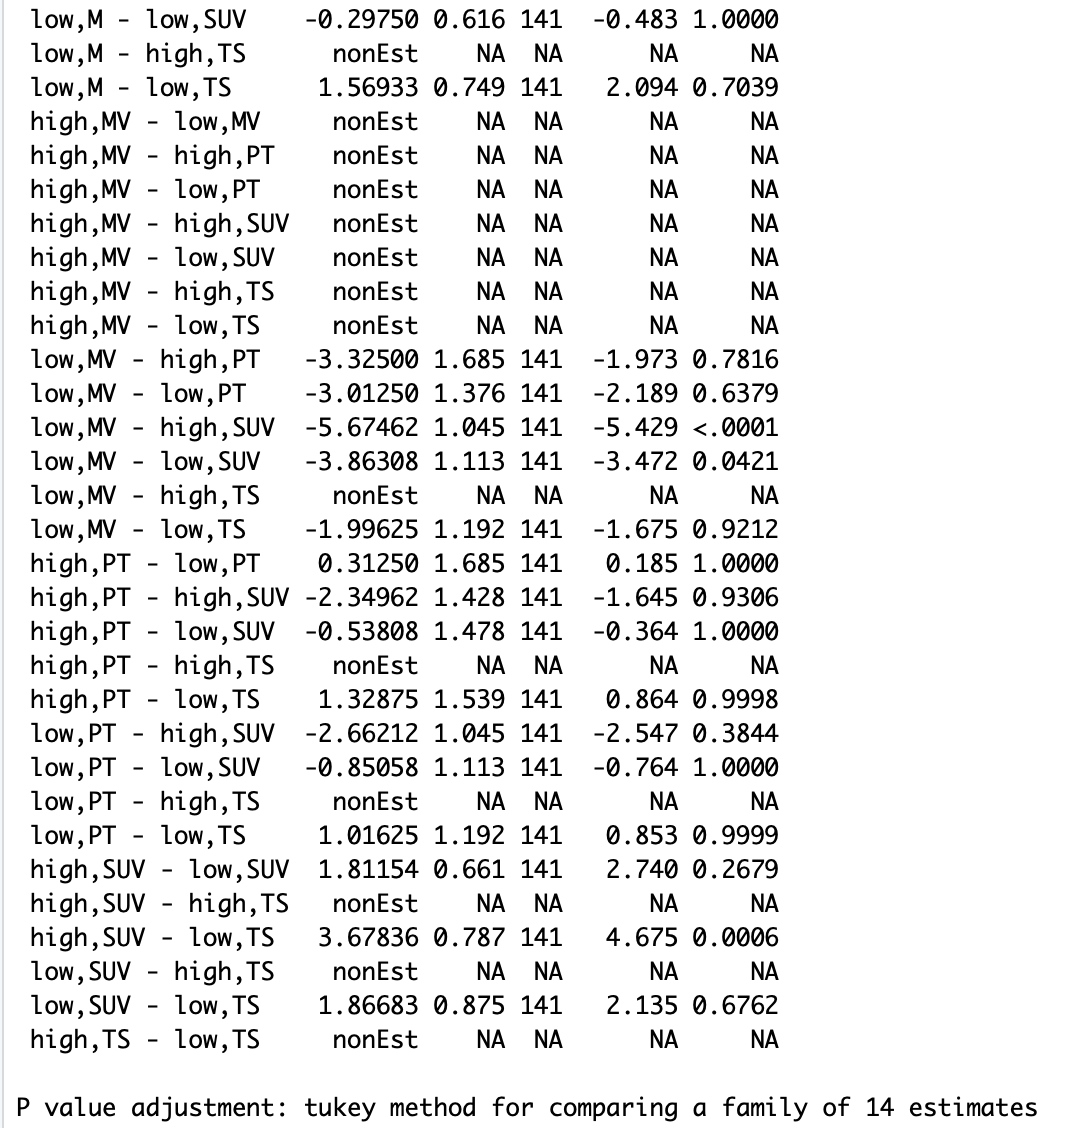
\includegraphics[width=0.48\textwidth]{../graphics/TWAcon3}}\\
		
		\hline
	\end{tabular}		
	\caption{Posthoc Test of Interactions.} %1
	\label{fig:PHT}
\end{figure}

\pagebreak
\section{SAS Code}
\lstinputlisting[
	caption=SAS Code (AppliedStatsProject.sas)., % Caption above the listing
	label=lst:SASCode, % Label for referencing this listing
	language=SAS, % Use SAS functions/syntax highlighting
	frame=single, % Frame around the code listing
	showstringspaces=false, % Don't put marks in string spaces
	numbers=left, % Line numbers on left
	numberstyle=\tiny, % Line numbers styling
	]{../code/AppliedStatsProject.sas}	
\pagebreak

\section{R Code}
\lstinputlisting[
	caption=R Code (AppliedStatsProject.R)., % Caption above the listing
	label=lst:RCode, % Label for referencing this listing
	language=R, % Use SAS functions/syntax highlighting
	frame=single, % Frame around the code listing
	showstringspaces=false, % Don't put marks in string spaces
	numbers=left, % Line numbers on left
	numberstyle=\tiny, % Line numbers styling
	]{../code/AppliedStatsProject.r}	
\bibliography{mybib}

\end{document}